\documentclass[twocolumn,onesided,9pt]{article}

\PassOptionsToPackage{table}{xcolor}

\usepackage{./Task32FlyerLatexStyle/Task32Flyer}
\usepackage{todonotes}

%% -----------------------------------
%% Document information
%% -----------------------------------
\def\pubdate{26 November 2020}
\title{2020 General Meeting}
\shorttitle{2020 General Meeting}
\doctype{IEA Wind Task 32 Meeting Minutes}
\DOI{10.5281/zenodo.4292208}
\addbibresource{bibliography.bib}

%% -----------------------------------
%% Style modifications (doc specific)
%% -----------------------------------
% task 32 action box
\usepackage{tcolorbox}
\newtcolorbox{taskactions}[1][]
{
	every float=\centering,
	width=1.0\columnwidth,
	boxsep=0pt,
	left=3pt,
	right=3pt,
	top=3pt,
	colframe = Task32Blue2,
	#1,
}
% no indents
\setlength{\parindent}{0pt}
% long tables
\usepackage{supertabular}
% define figure and section references
\newcommand{\fref}[1]{Fig.~\ref{#1}}
\newcommand{\sref}[1]{\S~\ref{#1}}
% set the TOC depth
\setcounter{tocdepth}{2}
% reduce spacing in TOC
\usepackage[titles]{tocloft}
\setlength{\cftbeforesecskip}{3pt}
% authors
\newcommand{\orcid}[1]{\href{https://orcid.org/#1}{
\includegraphics[width=12pt]{graphics/ORCIDiD_icon128x128.png}}}
\usepackage{fontawesome}
\newcommand{\mailme}[1]{\href{mailto:#1}{\faicon{envelope-o}}}

%% ===================================
%:
%% Document starts
%% ===================================
\begin{document}

%% -----------------------------------
%% Title
%% -----------------------------------
\maketitle
\thispagestyle{cover}

%% -----------------------------------
%% Authors
%% -----------------------------------
\noindent\begin{minipage}{\columnwidth}
\textcolor{TextLightGrey}{Authors: Andrew Clifton~\orcid{0000-0001-9698-5083}~\mailme{clifton@ifb.uni-stuttgart.de}, %
Ines Würth~\orcid{},
David Schlipf~\orcid{}}
\end{minipage}
\vskip 6pt

%% -----------------------------------
%% Introductory text
%% -----------------------------------
{\Large\noindent%
	Task 32 has created a worldwide network of wind lidar researchers who meet regularly to identify opportunities for the use of wind lidar, and mitigate the barriers to its adoption.
}
\vskip 6pt

The 2020 General Meeting took place online because of the COVID-19 pandemic.  COVID-19 made networking and collaboration harder for everyone during 2020, and so the 2020 General Meeting was designed to let the wind lidar community mingle virtually with their colleagues through a mix of discussion, working groups, and networking sessions.

\tableofcontents

\section*{Disclaimer}
The presence of a person’s name or company name in this document should not be taken to imply that a person or their employer agrees with any of the opinions set out here.

\newpage
\section{Day 1: Tuesday 20 October}

\begin{table}[!h]
 \centering
 % set up banded rows for the agenda and add lines to the columns
 \arrayrulecolor{Task32Blue2!15}
 \rowcolors{2}{Task32Blue2!5}{white}
 \begin{tabular}{@{}|p{0.125\columnwidth}|p{0.85\columnwidth}|@{}}
 \rowcolor{Task32Blue2} \textbf{Time} & \textbf{Activity} \\
 14:00 & Panel session on “Wind Lidar in 5 years”
  \begin{itemize}
        \item Alex Woodward, ZX Lidars
        \item Alexandra St. Pe, RWE
        \item Rozenn Wagner, GE Offshore Wind
        \item Reesa Dexter, DNV-GL
    \end{itemize} \\
 14:55 & Break \\
 15:00 & Working groups: creative chaos to make progress on something\\
 15:55 & Break \\
 16:00 & Networking session\\
 16:45 & Close \\
 \end{tabular}
 \label{tab:day1-agenda}
\end{table}

\subsection{Panel discussion: “Wind lidars in 5 years”}

We started with presentations from all panelists with their view of where wind lidars will be in 5 years. 68 people joined us for this session.

\subsubsection{Presentations}
Alex Woodward:
\begin{itemize}
    \item What if lidar manufacturers developed a really cheap lidar sensor? What would the community do with such a sensor? 
    \item What if there were lidars that can be customized, e.g., with apps that community experts would develop? What would you do with a smart lidar?
\end{itemize}
Reesa Dexter
\begin{itemize}
    \item Power performance with nacelle mounted lidar will be common
    \item Preference to used lidar over tall masts in simple terrain. R\&D on lidar in complex terrain will continue
    \item Better FLS uncertainties
    \item “wind tunnel” equivalent calibration of lidar instead of mast verifications
    \item Ability to measure across the rotor for the tallest of turbines    
\end{itemize}
Rozenn Wagner
\begin{itemize}
    \item Nacelle lidar will be the standard for power curve testing
    \item Lidars will be standard for resource and site assessment. The main challenge to be solved are turbulence intensity (TI) measurements
\end{itemize}
Alexandra St. Pé
\begin{itemize}
    \item Wind resource assessment
    \begin{itemize}
        \item How does varying TI input impact wake models?
        \item What's the impact of lidar speed and TI on $P\textrm{50}$ estimates?
    \end{itemize}
    \item Site suitability 
    \begin{itemize}
        \item How does TI impact load models?
        \item How does different load model output impact site suitability decisions?
    \end{itemize}
    \item Power performance tests
    \begin{itemize}
        \item How can power performance be more accurately and precisely be predicted using a lidar?
    \end{itemize}
    \item Performance monitoring
    \begin{itemize}
        \item How can we develop more integrated and intelligent wind farms?
        \item How can lidars be used to optimize turbine performance?
    \end{itemize}
\end{itemize}

\subsubsection{Discussion}
\emph{Many of the following questions and chat were taken verbatim from the video chat window. There have been some edits for spelling and clarity.}

Alex: ZX lidar carry out factory acceptance tests and for certain customers an met mast validation is carried out. For ZX the factory tests are much more important, and the field validation is an add-on. What would be needed to remove the need for a mast validation?
\begin{itemize}
    \item Rozenn: part of the answer is in the uncertainty estimation since the goal is to reduce the risk. And that is what is usually looked for in a validation. 
    \item Reesa: there needs to be an industry standard. It would be nice for the lidar manufacturer to have a standard way of coming up with an uncertainty quantification. We need industry acceptance. 
    \item Alexandra: the question is, why are we comparing to a cup? Cup-free validation would be ideal.
\end{itemize}

A researcher: a question to Reesa and Rozenn: How urgently does the industry really need TI measurements? How much do you think industry would be willing to pay for it as an extra?
\begin{itemize}
    \item Reesa: there’s been different stakeholders; OEMs, developers, and academia. There was a lot of great but technical work from academia. Industry needs more practical solutions. Masts cannot keep up with the high hub heights, so there is an economic incentive to resolve this. It is a bottleneck to move away from the cup and towards only lidar. It is an important part of moving the technology forward. 
    \item Alexandra: There has been a lot of work done. There is a gap in benchmarking all the methods. How do I know which method to use for a specific site and a specific lidar? I need something that is practical and does not cost much time. There is a Consortium for the Advancement of Remote Sensing (CFARS) \enquote{site suitability} subgroup that works with a lot of stakeholders and works on how to get lidar TI accepted for site suitability. We need to go from TI measurements also to loads models. We are coming to an end of the line. 
    \item Alex: the progress that CFARS and other groups are making is brilliant. The challenge as a lidar manufacturer is that we don't own the data; it's owned by the turbine OEM. The different groups are pushing now independently and CFARS can bring the acceptance over the tipping point. 
\end{itemize}

An industry engineer: how would a lidar sensor compare to a 3D ultrasonic anemometer? For example, if we were to estimate turbulent kinetic energy (TKE)?
\begin{itemize}
    \item Reesa: the primary driver is the volume that is being measured in. Lidars measure over a big volume compared to a sonic. Comparing sonics to lidar measurements, the sonics are more similar than cups. Cups have also issues, e.g. with overspeeding. 
\end{itemize}

A consultant: a question to Reesa/Rozenn: We already have quite some evidence for ground-based lidar (GBL) vs met mast TI measurements and the level of overestimation of GBL. Do you have some preliminary estimates on TI measurements from nacelle-mounted lidar? Do we expect it to be conservative compared to the GBL case, considering today's technology?
\begin{itemize}
    \item Rozenn: DTU have done a lot of analysis of this. Nacelle-mounted lidar would be less conservative than GBL. It is not the same bias because it is measured into the wind and is aligned to the yawing of the turbine. There is no simple correction to correct the TI, we still need to find a proper way to do that.
\end{itemize}

A lidar supplier: a question to Rozenn: you mentioned we need to measure wind profiles for PPT for large wind turbines. Could you elaborate? Would it be used to normalize the power curve, or determine if the shear value is within the range of the warranty power curve?
\begin{itemize}
    \item Rozenn: for me the ideal method would be to fulfill the requirements for rotor equivalent measurements. That means measuring at least at three heights, and at 2.5 diameters (2.5$D$) upstream. 
    \item Q: can you give details on the near measurements that you talked about?
    \item Rozenn: I am being conservative. I doubt we have overcome the 2.5$D$ challenge, so I think we need to measure the profile at that distance for 5 years.
\end{itemize}


\subsection{Working session}

\begin{table}[!h]
    \centering
    % set up banded rows for the agenda and add lines to the columns
    \arrayrulecolor{Task32Blue2!15}
    \rowcolors{2}{Task32Blue2!5}{white}
    \begin{tabular}{@{}
        |p{0.175\columnwidth-2\tabcolsep}
        |p{0.825\columnwidth-2\tabcolsep}
        |@{}}
    \rowcolor{Task32Blue2} \textbf{Time} & \textbf{Activity} \\
    15:00 & Working groups: creative chaos to make progress on something \\
    15:55 & Break \\
    \end{tabular}
    \label{tab:day1-workingsession-agenda}
\end{table}

63 participants split into self-selected groups. The group's outcomes are minuted in \hyperref[sec:reporting]{day 3}.

\subsection{Networking session}

\begin{table}[!h]
    \centering
    % set up banded rows for the agenda and add lines to the columns
    \arrayrulecolor{Task32Blue2!15}
    \rowcolors{2}{Task32Blue2!5}{white}
    \begin{tabular}{@{}
        |p{0.175\columnwidth-2\tabcolsep}
        |p{0.825\columnwidth-2\tabcolsep}
        |@{}}
    \rowcolor{Task32Blue2} \textbf{Time} & \textbf{Activity} \\
    16:00 & Networking session \\
    16:55 & Close \\
    \end{tabular}
    \label{tab:day1-networking}
\end{table}

Three rounds of random, 3-person breakout rooms were held. The day closed at 16:55 CEST.
\newpage
\section{Day 2: Wednesday 21 October}

\begin{table}[!h]
    \centering
    % set up banded rows for the agenda and add lines to the columns
    \arrayrulecolor{Task32Blue2!15}
    \rowcolors{2}{Task32Blue2!5}{white}
    \begin{tabular}{@{}
        |p{0.175\columnwidth-2\tabcolsep}
        |p{0.825\columnwidth-2\tabcolsep}
        |@{}}
    \rowcolor{Task32Blue2} \textbf{Time} & \textbf{Activity} \\
    14:00 & Panel session on “Wind lidar - I wish we knew how to...”:
        \begin{itemize}
            \item Mads V. Sorensen, EMD
            \item Peter Rosenbusch, Leosphere
            \item  Zachary Parker, Nordex
            \item Julia Gottschall, Fraunhofer IWES
        \end{itemize} \\
    14:55 & Break \\
    15:00 & Working groups \\
    15:55 & Break \\
    16:00 & Community news: 
        \begin{itemize}
            \item Update from the “wind lidar in cold climate” working group (Nicolas Jolin, Nergica)
            \item Update from the “wind lidar in complex terrain” working group (Alexander Stökl, Energiewerkstatt)
            \item A possible new round-robin on forward-looking lidar TI (Jens Riechert, DNV-GL)
        \end{itemize}\\
    16:45 & Close
    \end{tabular}
    \label{tab:day2-agenda}
\end{table}
\subsection{Panel discussion: \enquote{Wind lidar - I wish we knew how to...}}

We started with presentations from all panelists with their views
of where the entire wind energy and wind lidar community have work to
do. 52 people joined us.

\subsubsection{Presentations}

Mads V. Sorensen: I wish I knew how to get most value out of short (e.g. 3 months) measurement campaigns

\begin{itemize}
    \item in terms of TI, seasonality, shear
    \item why should one use a lidar if it is the same cost for 12 months than a mast
    \item why not use the full advantage of the lidar
\end{itemize}

Peter Rosenbusch: I wish WE knew how to\ldots{}

\begin{itemize}
    \item Eliminate the cup anemometer from the uncertainty budget
    \item Augment acceptance of ground-based lidars in complex terrain
    \item Establish nacelle lidar for PPT in complex terrain
    \item Optimize offshore WRA by combining floating lidar and lidar from the shore
    \item Establish best practice for site suitability with ground based lidars
\end{itemize}

Zachary Parker: I wish we knew how to\ldots{}

\begin{itemize}
    \item determine load assessment bias and uncertainty given remote sensing measurements
    \item validate, correct and use remote sensing data for load assessment → TI, shear and wind speed
    \item provide guidance from the turbine OEM perspective on the use (or not) of remote sensing
\end{itemize}

Julia Gottschall: I wish we knew how to\ldots{}

\begin{itemize}
    \item Do the optimal measurements (most likely with lidar)... in terms of chosen technology, setup, duration, requirements on accuracy and availability → what should we really measure?
    \item There are two necessary steps: 1, to understand application as well as possible and 2. to consider all possible data sources
\end{itemize}

\subsubsection{Discussions}

\emph{Many of the following questions and chat were taken verbatim from the video chat window. There have been some edits for spelling and clarity.}

Question from Julia: Should we put a scanning lidar on a buoy?

\begin{itemize}
\item  Peter Rosenbusch: I have no objections to this. We are involved in a
  research project. The definition of a scanning lidar is a device which
  can point the measurement to any point. A benefit of a scanning lidar
  is to be able to put it on the shore, or on the transition piece of a
  turbine.
\end{itemize}

From an industry researcher to Julia: Should we 'measure' turbulence using TI as currently defined involving the standard deviation over 600-second intervals, or is there some other way to 'measure' turbulence that would give a better input to models? Would TKE be better to use in conjunction with models?

\begin{itemize}
\item  Julia asks back: is it easier to work on the measurements or on the models? I personally don't know. We should not force a lidar to work as a cup because it cannot. We should understand the models and the measurements better. We also need to consider the bankability and the industry. My conclusion is we should try all of this, even a small impact will have a larger impact in the future. We should not be happy with using a lidar with a standard TI.
\item  Researcher: the measurement people stay with what they know and same for the load assessment people. Both groups should work together better. I think the load assessment process will be very difficult to change as it is based on many years of understanding of how to calibrate the load models. The new way of lidar measurement would require to throw away the existing experience. In the short term, you should adapt the measurements. In the long term, you should adapt the process.
\item  Peter: the calibration of the models to a point measurement seems less perfect in light of always growing turbines. 
\item Zachary: we see if we just use the lidar as a point measurement, we just get higher loads. We really need to understand first how to use the additional  information.
\item  David Schlipf: a lidar can give you a much better estimate over the whole rotor area than a cup anemometer could.
\end{itemize}

From an industry engineer to Mads and the group: Do we have a method to 'long-term' correct standard deviation / TI...from 3 months to 1 or multiple years? How to get the most out of your measurements?

\begin{itemize}
\item  Answer: Not really!
\item  Andy: this ties in to the presentations yesterday, especially from Reesa. We need to develop new tools, but the need for simple tools is very clear. We cannot treat this just as an academic problem, we need simple solutions.
\end{itemize}

Andy wants to come back to question of whether we get the most value out of a lidar, or could we do better?

\begin{itemize}
\item  Peter: I think we could do better. We are trying to optimize e.g. the position of the lidar. Do you have simulation tools to help you decide whether to put that?
\item  Mads: there are flow models that can help, but they come at a cost. If you're not sure you only start measuring at one point. I would like to take the idea of the modeling: to get the most out of lidar measurements, the effort should be on the modeling. E.g. you could throw information from several different measurements positions into a flow model and get better results.
\item  Zachary: the lidar can give you information on the stability, and this   is very important to get the modeling right.
\item  Julia: There are a lot of statistics of the wind fields involved, it is not just the modeling that is a challenge. So we should invest a lot of work in both. German guidelines will stick to 12 months for site assessment. I think it depends on the site. 
\item  Zachary: There are a lot of statistics coming out of the lidar, we should also look more at the raw data.
\item  Andy: We have made some progress in the last few years on measurements and modeling, but there is still a lot of work to do.
\end{itemize}

Folks who leave the meeting should do this..

\begin{itemize}
\item  Mads: consider the measurement period
\item  Julia: understand what your colleagues want to use the data for
\item  Zachary: study colocated lidar and sonic data with 1Hz
\item  Peter: brainstorm how to use the flexibility that a lidar provides
\end{itemize}
\subsection{Working session}

\begin{table}[!h]
    \centering
    % set up banded rows for the agenda and add lines to the columns
    \arrayrulecolor{Task32Blue2!15}
    \rowcolors{2}{Task32Blue2!5}{white}
    \begin{tabular}{@{}
        |p{0.175\columnwidth-2\tabcolsep}
        |p{0.825\columnwidth-2\tabcolsep}
        |@{}}
    \rowcolor{Task32Blue2} \textbf{Time} & \textbf{Activity} \\    
    15:00 & Working groups: creative chaos to make progress on something \\
    15:55 & Break
    \end{tabular}
    \label{tab:day2-workingsession-agenda}
\end{table}

47 participants were split into 10 groups based on the preferences indicated before the meeting and in the break. The working groups were not minuted, but the outcomes are available in the minutes for day 3.

\subsection{Community news}

\begin{table}[!h]
  \centering
  % set up banded rows for the agenda and add lines to the columns
  \arrayrulecolor{Task32Blue2!15}
  \rowcolors{2}{Task32Blue2!5}{white}
  \begin{tabular}{@{}|p{0.125\columnwidth}|p{0.85\columnwidth}|@{}}
  \rowcolor{Task32Blue2} \textbf{Time} & \textbf{Activity} \\  
  16:00 & Community news:
    \begin{itemize}
      \item The \enquote{wind lidar in cold climate} working group (Nicolas Jolin, Nergica)
      \item The \enquote{wind lidar in complex terrain} working group (Alexander Stökl, Energiewerkstatt)
      \item A possible new round-robin on forward-looking lidar TI (Jens Riechert, DNV-GL)
    \end{itemize}\\
  16:45 & Close \\
  \end{tabular}
  \label{tab:day2-community-news-agenda}
\end{table}

50 people joined us for an update on our ongoing activities.

\subsubsection[Update from the \enquote{wind lidar in cold climate} working group]{Update from the \enquote{wind lidar in cold climate} working group (Nicolas Jolin, Nergica)}

\emph{Nicolas presented an update on the \enquote{wind lidar in cold climate} working group. The presentation will be made available online.}

An industry researcher: how do you estimate the liquid water content from the CNR and how sure are you on your temperature profile? This would be very interesting.

\begin{itemize}
\item Nicolas: we do not have a clear method yet. We need to find the   correlation of the data with icing. One solution could also involve machine learning. We do not have a clear measure to extrapolate temperature profiles.
\end{itemize}

Andy: What would a good data set look like?

\begin{itemize}
\item Nicolas: The type of lidar does not matter. 1-2 months of 10-minute lidar data, temperature, and altitude information.
\end{itemize}

An industry researcher: what can we get out of CNR or the spectra that would help us with the question of liquid water?

\begin{itemize}
\item Paul Mazoyer: we did not work on that ourselves but with an institute   that worked on detecting icing. There are things possible, but we have not commercialised them.
\item Chris Slinger: the raw spectra is recorded and by eye you can tell if it is raining. There should be methods using this. At DTU Ana Maria Tilk is working on blade erosion.
\item Hans Jorgenson (DTU): Mikkel Seijhorn is working on this topic as well.
\end{itemize}

\subsubsection[Update from the \enquote{wind lidar in complex terrain} working group]{Update from the \enquote{wind lidar in complex terrain} working group (Alexander Stökl, Energiewerkstatt)}
\label{sec:news-complex-terrain-group}

An industry researcher: regarding the question of how to quantify terrain complexity: Have you considered the methodology described in Section 11.2 in IEC 61400-1:2019? (this describes a method for \enquote{Assessment of the topographical complexity})

\begin{itemize}
\item Alexander: yes they are a starting point, they give you a lower safe limit, but they do not tell you how far to go.
\end{itemize}

An industry wind lidar user: What is the reason for correcting the data for 'the effect of complexity'?

\begin{itemize}
\item Alexander: There are several methods used for lidar data correction on   a regular basis. One point is to have a look at the suitability of the  methods and how they compare to each other on these kinds of sites. It would have been nicer to have a broader range of sites to compare. We compare met mast data with lidar data. What we want to know is how good we get when applying the correction to the lidar data. 
\item Andy: wind lidar in complex terrain sometimes gives different estimates of wind speed and direction than a met mast. This is a result of the windfield reconstruction not capturing the true properties of the wind field (e.g. by incorrectly assuming flow homogeneity)
\item The user: alright, so the goal is to establish transfer functions between met mast and lidar.
\end{itemize}

An academic researcher: Where do the highest uncertainties come from when assessing lidar data in complex terrain?

\begin{itemize}
\item Alexander: you do not have a steady and homogeneous flow. When you decompose the signal from the different beams, you make an error because usually you use the assumption of homogeneity. If you use a flow model you can correct for it using a correction model.
\item The academic researcher: the wind field reconstruction is giving you the highest uncertainty.
\item Alexander: it is a complex problem!
\end{itemize}

\subsubsection[A possible round robin on turbulence estimates from nacelle-mounted lidar]{A possible new round-robin on turbulence intensity estimations from nacelle mounted lidar systems (Jens Riechert, DNV-GL)}

Jens presented details of a proposed round-robin.

The General Meeting participants were polled to ask if they would be interested in participating in the round robin:

\begin{itemize}
\item Yes, actively: 5
\item Yes, as an observer: 14
\item No: 9
\end{itemize}

A problem with the Zoom polling tool prevented some people from indicating that they would actively participate in the round robin. It is estimated that at least 5 votes for \enquote{yes, actively} were not cast, giving a total of 10 votes for \enquote{yes, actively}.

Q: What datasets are you looking for?

\begin{itemize}
\item Jens: the idea is to have both a pulsed and also a CW lidar exists. We would like a data set with simultaneous measurements with the same conditions.
\end{itemize}

\begin{taskactions}
\textbf{Task 32 action}: Task 32 will support this round robin and will work with Jens to hold a meeting later in 2020.
\end{taskactions}

\newpage
\section{Day 3: Thursday 21 October}

\begin{table}[!h]
    \centering
    % set up banded rows for the agenda and add lines to the columns
    \arrayrulecolor{Task32Blue2!15}
    \rowcolors{2}{Task32Blue2!5}{white}
    \begin{tabular}{@{}
        |p{0.175\columnwidth-2\tabcolsep}
        |p{0.825\columnwidth-2\tabcolsep}
        |@{}}
    \rowcolor{Task32Blue2} \textbf{Time} & \textbf{Activity} \\  
    14:00 & Panel session on “Wind lidar - the next generation”:
        \begin{itemize}
            \item Clym Stock-Williams, TNO
            \item Sandrine Aubrun, ECN
            \item Marijn Floris van Dooren, ForWind, Oldenburg
            \item Sarah Barber, OST
        \end{itemize} \\
    14:55 & Break \\
    15:00 & Working groups \\
    15:55 & Break \\
    16:00 & Reporting \& next steps \\
    16:45 & Close
    \end{tabular}
    \label{tab:day2-agenda}
\end{table}
\subsection{Panel discussion: \enquote{Wind lidar - the next generation}}

We started with presentations from all panelists with their view of how the wind lidar and wind energy community should be teaching and training the next generation of wind lidar users. 53 participants joined us for this session.

\subsubsection{Presentations}

Clym Stock-Williams, TNO

\begin{itemize}
	\item Scientist in industry must know the limitations and assumptions of their equipment, especially for lidar systems
	\item Regular training courses on lidar related technology are needed targeted at industry professionals
	\item Data scientists and statisticians are largely missing from wind energy industry
\end{itemize}

Sandrine Aubrun, ECN

\begin{itemize}
	\item Do not set meteorology and engineering sciences as opposites or exclusives in education programs - both subjects are important but are taught in different courses
	\item Better transfer of knowledge from the research community to the industrial end-users
\end{itemize}

Marijn Floris van Dooren, ForWind

\begin{itemize}
	\item Should lidar theory and wind energy application be an integral part of uni programs?
	\item Do we need a lidar course for a non-academic audience?
	\item Existing European/international networks such as the European Wind Energy Master and the ITN project LIKE push the expertise and exploitation of lidar and enhance diversity in the field.
\end{itemize}

Sarah Barber, OST

\begin{itemize}
	\item Improving diversity in wind energy science
	\item Why do we need to improve diversity? The workforce does not represent our population's diversity which results from inequality
	\item Why should I care? Diverse teams are more productive
	\item What can I do? Increase awareness, get clued up, observe and report discriminations
\end{itemize}

\subsubsection{Discussions}

\emph{Many of the following questions and chat were taken verbatim from the video chat window. There have been some edits for spelling and clarity.}

Sarah to Sandrine: How should we set up those programs?

\begin{itemize}
	\item Sandrine: We have to actively facilitate transfer of knowledge. This could be a task for the LIKE project.
	\item Peter Rosenbusch: I am very grateful for the collaboration between academia and industry. A technology workshop is ongoing. We are offering webinars at Leosphere, and are happy to do more of those.
	\item Marijn: There are two industry workshops planned in LIKE where the goal is to transfer knowledge between the groups. One project might not be enough!
\end{itemize}

Andy to Clym: are we reaching enough people, or is the lidar community too small?

\begin{itemize}
	\item Clym: it is great to hear that industry if offering courses. But the question is, if those courses also teach others' technology. Wind field reconstruction is a very important topic as well that needs to be taught. And each device needs to be treated differently.
\end{itemize}

Question from the chat: Why is knowledge of wind energy not so open and accessible in online platforms like Coursera or EDX, compared to solar energy? I know this is something irrelevant to current discussion but I would love to hear from current members?

\begin{itemize}
	\item From Sarah Barber (via chat): Hi \ldots, this is a really good question and very relevant to the topic, in my opinion. We at OST are
 actually involved in trying to solve this problem by building a wind energy collaboration platform including data and workflow sharing. I can tell you more about it in private if you are interested. 
	 \item Zachary - I wonder if a collaboration with IEA Wind Task 43 Digitalisation might be interesting for this? Data sharing and collaboration is a part of this task.
	\item From Sandrine: I think this is a very good idea. This should be the objective of the EAWE (European Academy for Wind Energy) or other academic institutions. Such a course could be the goal to be constructed.
	\item Sarah: there are not many wind energy courses. So it is not surprising that there is nothing online so far. The question might also be, if we need more of those basic courses
	\item Marijn: I agree, there are not many programs. In Oldenburg there are good courses, but this is not part of a specialization. The European Wind Energy Master program (EWEM is a collaboration between TU Delft, DTU, NTNU, and the University of Oldenburg) is a successful example of how knowledge can be combined within Europe. But more combined or shared programs would be good.
	\item Clym: There might be a difference between solar and wind because solar is more for domestic use. A wind energy master would be extremely useful for a university. In Delft there is also a course that has to be paid for. In my experience the students from master courses have a broad knowledge. A basic bachelor knowledge and a master in wind is often not enough knowledge to go into research. The specialization should take place on PhD level.
	\item Andy: for lidar we need to come up with material that sums up the state of the art.
	\item David: Master students are often looking for topics but cannot find some. The Task 32 could offer to be a platform for advertising master thesis topics in the newsletter
	\item Zachary responded: Like the one I recently posted on Linkedin!
\end{itemize}

Question from the chat: This seems to be a matter of managing interfaces. Research sometimes needs to be separate from industry to encourage innovation without certain limits, and then it needs to exchange at a certain point to be used practically. How can we use IEA Task 32 to guide/frame the interface?

\begin{itemize}
	\item Marijn: indeed this interface is missing. Often practicalities make it very hard to test things or implement ideas
	\item Andy: We need playgrounds where industry and academia can meet safely on a legal basis.
	\item Sarah: we need a way for industry and academia to work together with common data. I think it is possible to have a platform or set up where this is possible.
	\item Andy: we are starting to ask questions about digitalisation of lidar. We will be spinning this up over the next year.
\end{itemize}

Question from the chat: LiDAR technology for wind originally came from the atmospheric boundary layer research community. Today, the wind energy science community is somehow \enquote{separated} (maybe not the right term) from the ABL research world (with some exceptions like the collaboration with DWD for \href{https://www.windfors.de/en/projects/wipaff/}{WIPAFF}). Do you think it would make sense to reconnect with the ABL met folks, for instance through projects like the EU \href{https://www.cost.eu/actions/CA18235/\#tabs\%7CName:overview}{PROBE COST Action}? They have wind lidars too, but also use lidars for other things, and have other interesting tech like radiometers for instance. How much overlap do you think with those groups?

\begin{itemize}
	\item Sandrine: I think this is exactly the idea which I had for the educational program which is split between earth sciences and engineering. A lot of people in wind energy a lot of people come from physics or earth science - so the link exists already but is probably not used enough or established.
	\item Andy: Often we are most comfortable to talk to people who are doing something similar. The Task 32 OA is trying to get involved with PROBE but this may take some time. We encourage everyone to get involved with other activities where they see links and share knowledge from, or with, Task 32.
\end{itemize}

Andy: This brings us back to diversity. Sarah brought up the point, that if you don't have the whole society represented, you do not get what you need. Do you think we are wearing a white western hat?

\begin{itemize}
	\item Sarah: Well, you are wearing a white male, western european heterosexual hat. And that is unconscious. Everybody should be conscious about it.
	\item Andy: as white male engineers - what might I be doing that stops different people from engaging?
	\item Sarah: Starts with language. A lot of people refer to engineers as he. You might write a job description which focuses more on male behaviours. I had a job description myself recently with only male applications. And so the topic might be not written in an interesting way to appeal to female people.
\end{itemize}

Andy to all participants: what was your experience with trying to get a diverse applicant pool into your projects?

\begin{itemize}
	\item Marijn: All universities tried to take care of diversity, and the \href{https://www.msca-like.eu/}{ITN LIKE} project is relatively diverse.
	\item Sandrine: in FLOAWER we tried to increase the percentage of accepted women compared to how many applied. The key element of selection was not the gender but the knowledge. We still managed to improve the percentage. I got feedback from positive discremination by being too many women in my group. Sometimes we are being used as representatives. For my career this was a positive aspect.
	\item Ines agrees: It is important to start early. For example at the University of Stuttgart girls from school are introduced to science at an early age through the \href{https://www.uni-stuttgart.de/studium/orientierung/try-science/}{Try Science} program.
	\item Clym: how can we help as a lidar community? My feeling for outreach work is that lidar is a very physical subject. Everyone experiences the wind, the magic of lidar ist that you can feel it. And this is inspiring. There is an african society which is also trying to foster diversity - so we should really try to reach out of our own borders.
\end{itemize}

An engineer (via chat): Hiring practices need to be less intuition based - see e.g., \enquote{Thinking, Fast and Slow} Chapter 21, by Daniel Kahnemann\cite{kahneman2011thinking}. What role could IEA Task 32 really play in encouraging this?

\begin{itemize}
	\item Sarah Barber: The first step is even getting people to accept that under-representation \emph{is} a problem. Many people do \emph{not} believe that something has to be done, because encouraging under-represented groups is seen as \enquote{positive discrimination} or discriminating \emph{against} the white male.
\end{itemize}

Andy: What would the panel members like to provide as a \enquote{take away}?

\begin{itemize}
	\item Marijn: We as a lidar community should make sure that we provide a safe environment for everybody
	\item Sarah: Increasing diversity is something we can do every day - let's get started.
\end{itemize}

\begin{taskactions}
\textbf{Task 32 action}: we will:

\begin{itemize}
	\item Encourage all of our members to get in contact if they would like to use our LinkedIn feed or newsletter to advertise open positions.
	\item Explore the need for structured further education that can be supported by the Task.
	\item look at our activities again from the perspective of diversity and inclusion to make sure that we encourage and enable everyone to take part in the Task. If any of our members have comments, questions, or critique, please \href{mailto:ieawind.task32@ifb.uni-stuttgart.de}{contact the Operating Agents}.
\end{itemize}
\end{taskactions}
\subsection{Working session}

\begin{table}[!h]
    \centering
    % set up banded rows for the agenda and add lines to the columns
    \arrayrulecolor{Task32Blue2!15}
    \rowcolors{2}{Task32Blue2!5}{white}
    \begin{tabular}{@{}
        |p{0.175\columnwidth-2\tabcolsep}
        |p{0.825\columnwidth-2\tabcolsep}
        |@{}}
    \rowcolor{Task32Blue2} \textbf{Time} & \textbf{Activity} \\    
    15:00 & Working groups: creative chaos to make progress on something \\
    15:55 & Break
    \end{tabular}
    \label{tab:day2-workingsession-agenda}
\end{table}

47 participants split into 8 groups based on the preferences indicated before the meeting and in the break. The working groups were not minuted directly, but the outcomes are available in the next section.

\subsection{Reporting and next steps}
\label{sec:reporting}

\begin{table}[!h]
    \centering
    % set up banded rows for the agenda and add lines to the columns
    \arrayrulecolor{Task32Blue2!15}
    \rowcolors{2}{Task32Blue2!5}{white}
    \begin{tabular}{@{}
        |p{0.175\columnwidth-2\tabcolsep}
        |p{0.825\columnwidth-2\tabcolsep}
        |@{}}
    \rowcolor{Task32Blue2} \textbf{Time} & \textbf{Activity} \\    
    16:00 & Reporting and next steps \\
    16:55 & Break
    \end{tabular}
    \label{tab:day4-results-agenda}
\end{table}

43 participants joined us to hear about the outcomes from the working groups.

Each group was allocated 1 slide and 3 minutes to present their work. Each group appointed a rapporteur to present their work.

Following are the notes from each group including the summary slide that they prepared. The slides have been reproduced without editing.

\subsubsection{Forecasting}

\emph{Rapporteur: Ines Würth}

This is a topic with lots of open questions, but there's not much public research in this area at the moment. Task 32 remains a great place to share ideas. %More information about the discussion in this group is available in the \href{https://docs.google.com/document/d/1Yq2JyWJAEZVAJE9te4FJ-57OpXdxNRHWhks88l2YJcI/edit?usp=sharing}{working group's notes}.

\begin{taskactions}
\textbf{Task 32 action}: we'll store those open questions in a public space and make them available for others to build on.
\end{taskactions}

\subsubsection{Wind lidar for wind energy applications in cold climate}

\emph{Rapporteur: Nicolas Jolin}

See the presentation from Day 2 for more information about this working group. Studies are ongoing. Please get in contact with Nicolas Jolin if you are interested.

\begin{taskactions}
\textbf{Task 32 action}: Task 32 will continue to support this working group.
\end{taskactions}

\subsubsection{A world without cups}

\emph{Rapporteur: Mads Sorensen, Remi Gandoin}

\begin{itemize}
\item These were more philosophical discussions. But it's important to think about philsophy when looking into the future.
\item An entire industry needs to be changed!
\item the laser technology and the great progress it lead to in physics;
\item going beyond the \enquote{lidars don't give me TI} concerns and approach by questioning/better understanding what these TI values are used for (typically to evaluate the IEC turbulence class). In effect, in the IEC framework, the input flow models that are used for the load simulations are really \enquote{toy} models of the atmosphere (i.e., steady-state over 10 minutes, power law shear, and Kaimal neutral form spectra with pre-defined length scales). Despite the potential of wind lidar, we are missing practical examples of situations where LiDARs lead to better siting/WTG choice than cups.
\end{itemize}

\begin{taskactions}
\textbf{Task 32 action}: Task 32 will continue to explore this question. We may identify a work case that is not well-served by cup anemometers and the current approach to wind characterisation, and investigate how to leverage wind lidar instead.
\end{taskactions}

\subsubsection{Collaboration on wind lidar hardware and software}

\emph{Rapporteur: Francisco Costa}

There's a lot of work going on in this area. The major challenge is to coordinate activities and tools, and enable them to work together (\fref{fig:day3-collaboration-hardware-software}).

% \begin{figure*}[p]
% \centering
% \fbox{
% 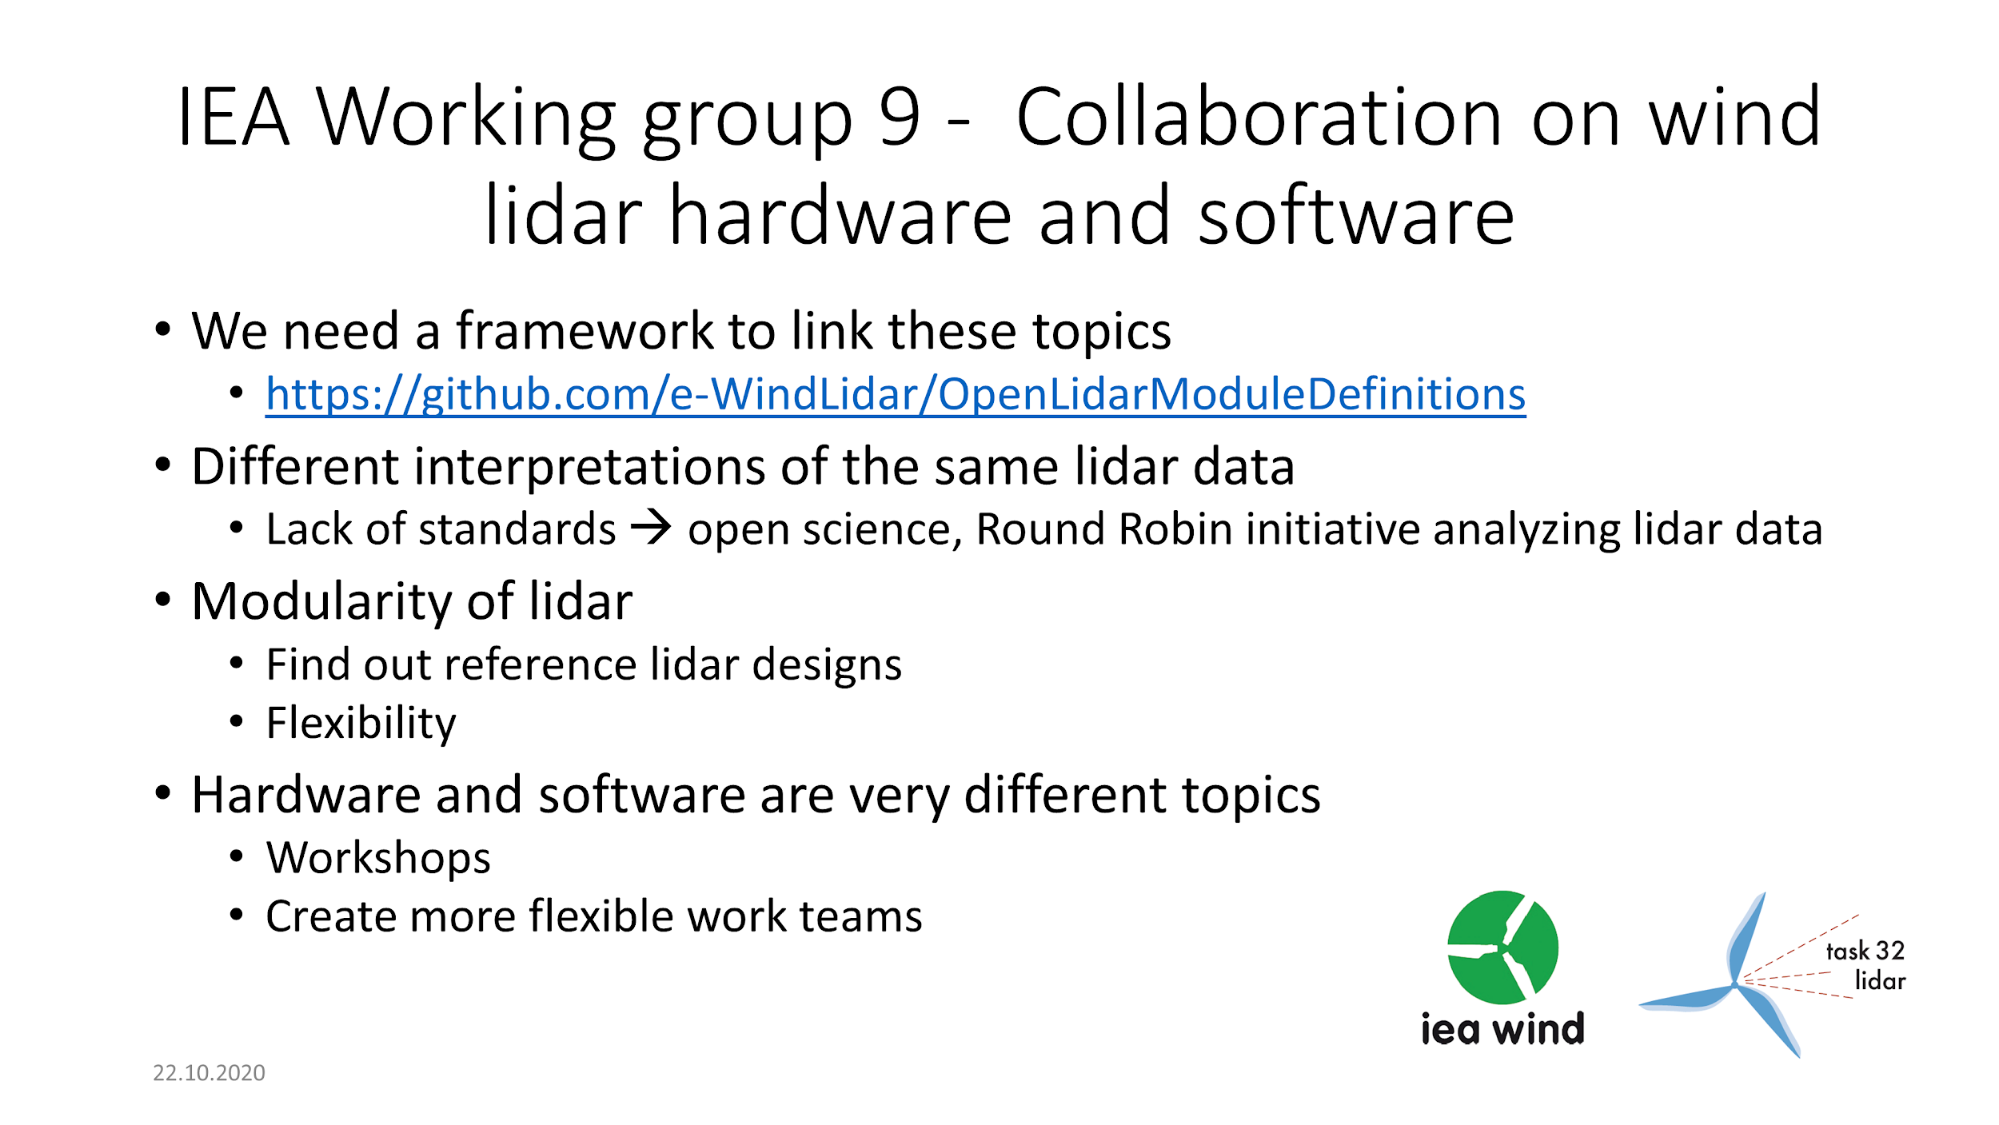
\includegraphics[width=0.85\textwidth]{figures/day3-collaboration-hardware-software.png}
% }
% \caption{Collaboration on wind lidar hardware and software}
% \label{fig:day3-collaboration-hardware-software}
% \end{figure*}
\begin{taskactions}
\textbf{Task 32 action}: we'll update the \href{https://github.com/IEA-Wind-Task-32/wind-lidar-glossary}{Task 32 Glossary} to include a generic lidar design approach that is aligned with the open lidar modular concept \cite{clifton_2019_openlidar}. This glossary can be used to define classes for lidars, like \emph{optics.telescope.aperture} which could help with defining inputs for simulations, etc. We'll also create reference designs using this structure.
\end{taskactions}

\subsubsection{Turbulence intensity derived from wind lidar}

\emph{Rapporteur: Reesa Dexter}

This has been a recurrent theme through the General Meeting. There are opportunities to go beyond current approaches to just mirror conventional met masts (\fref{fig:day3-Ti-group}). A workshop bringing industry and academia together would be a good next step.

% \begin{figure*}[p]
%     \centering
%     \fbox{
%     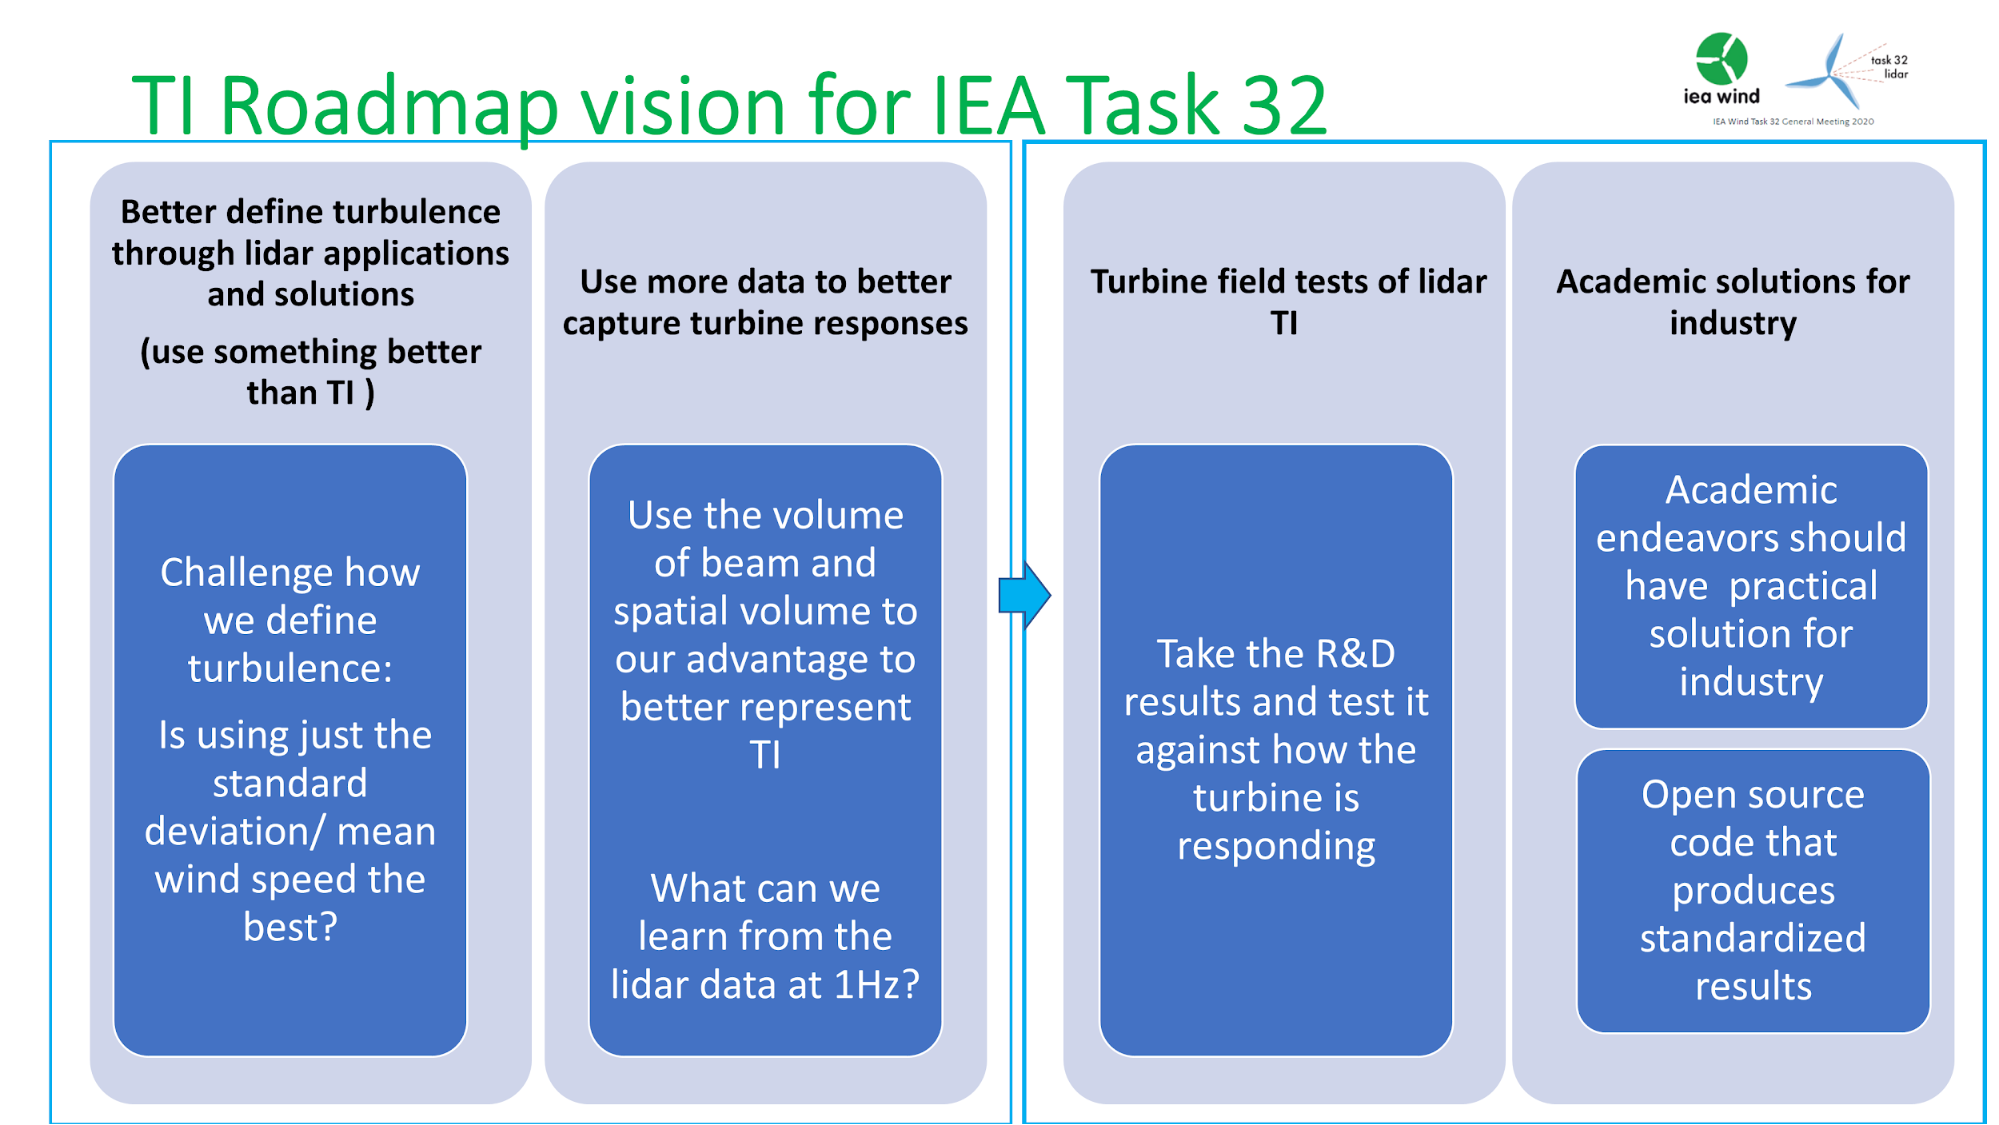
\includegraphics[width=0.85\textwidth]{figures/day3-Ti-group.png}
%     }
%     \caption{A lidar-derived turbulence data roadmap vision for Task 32 }
%     \label{fig:day3-Ti-group}
% \end{figure*}

\begin{taskactions}
\textbf{Task 32 action}: we'll include the suggested next steps in our roadmap and start to plan events for 2021 and beyond. We'll also coordinate with CFARS.
\end{taskactions}

\subsubsection{Wind lidar in complex terrain}

\emph{Rapporteur: Alexander St\"okl}

There continues to be a lot of interest in the potential to use wind lidar in complex terrain. This means we need tools to do it reliably and predictably, and we need to know when we hit the limits of our capabilities (\fref{fig:day3-complex-terrain}). There's an active Task 32 working group in this area, led by Alexander (see \sref{sec:news-complex-terrain-group}.)

% \begin{figure*}[p]
%     \centering
%     \fbox{
%     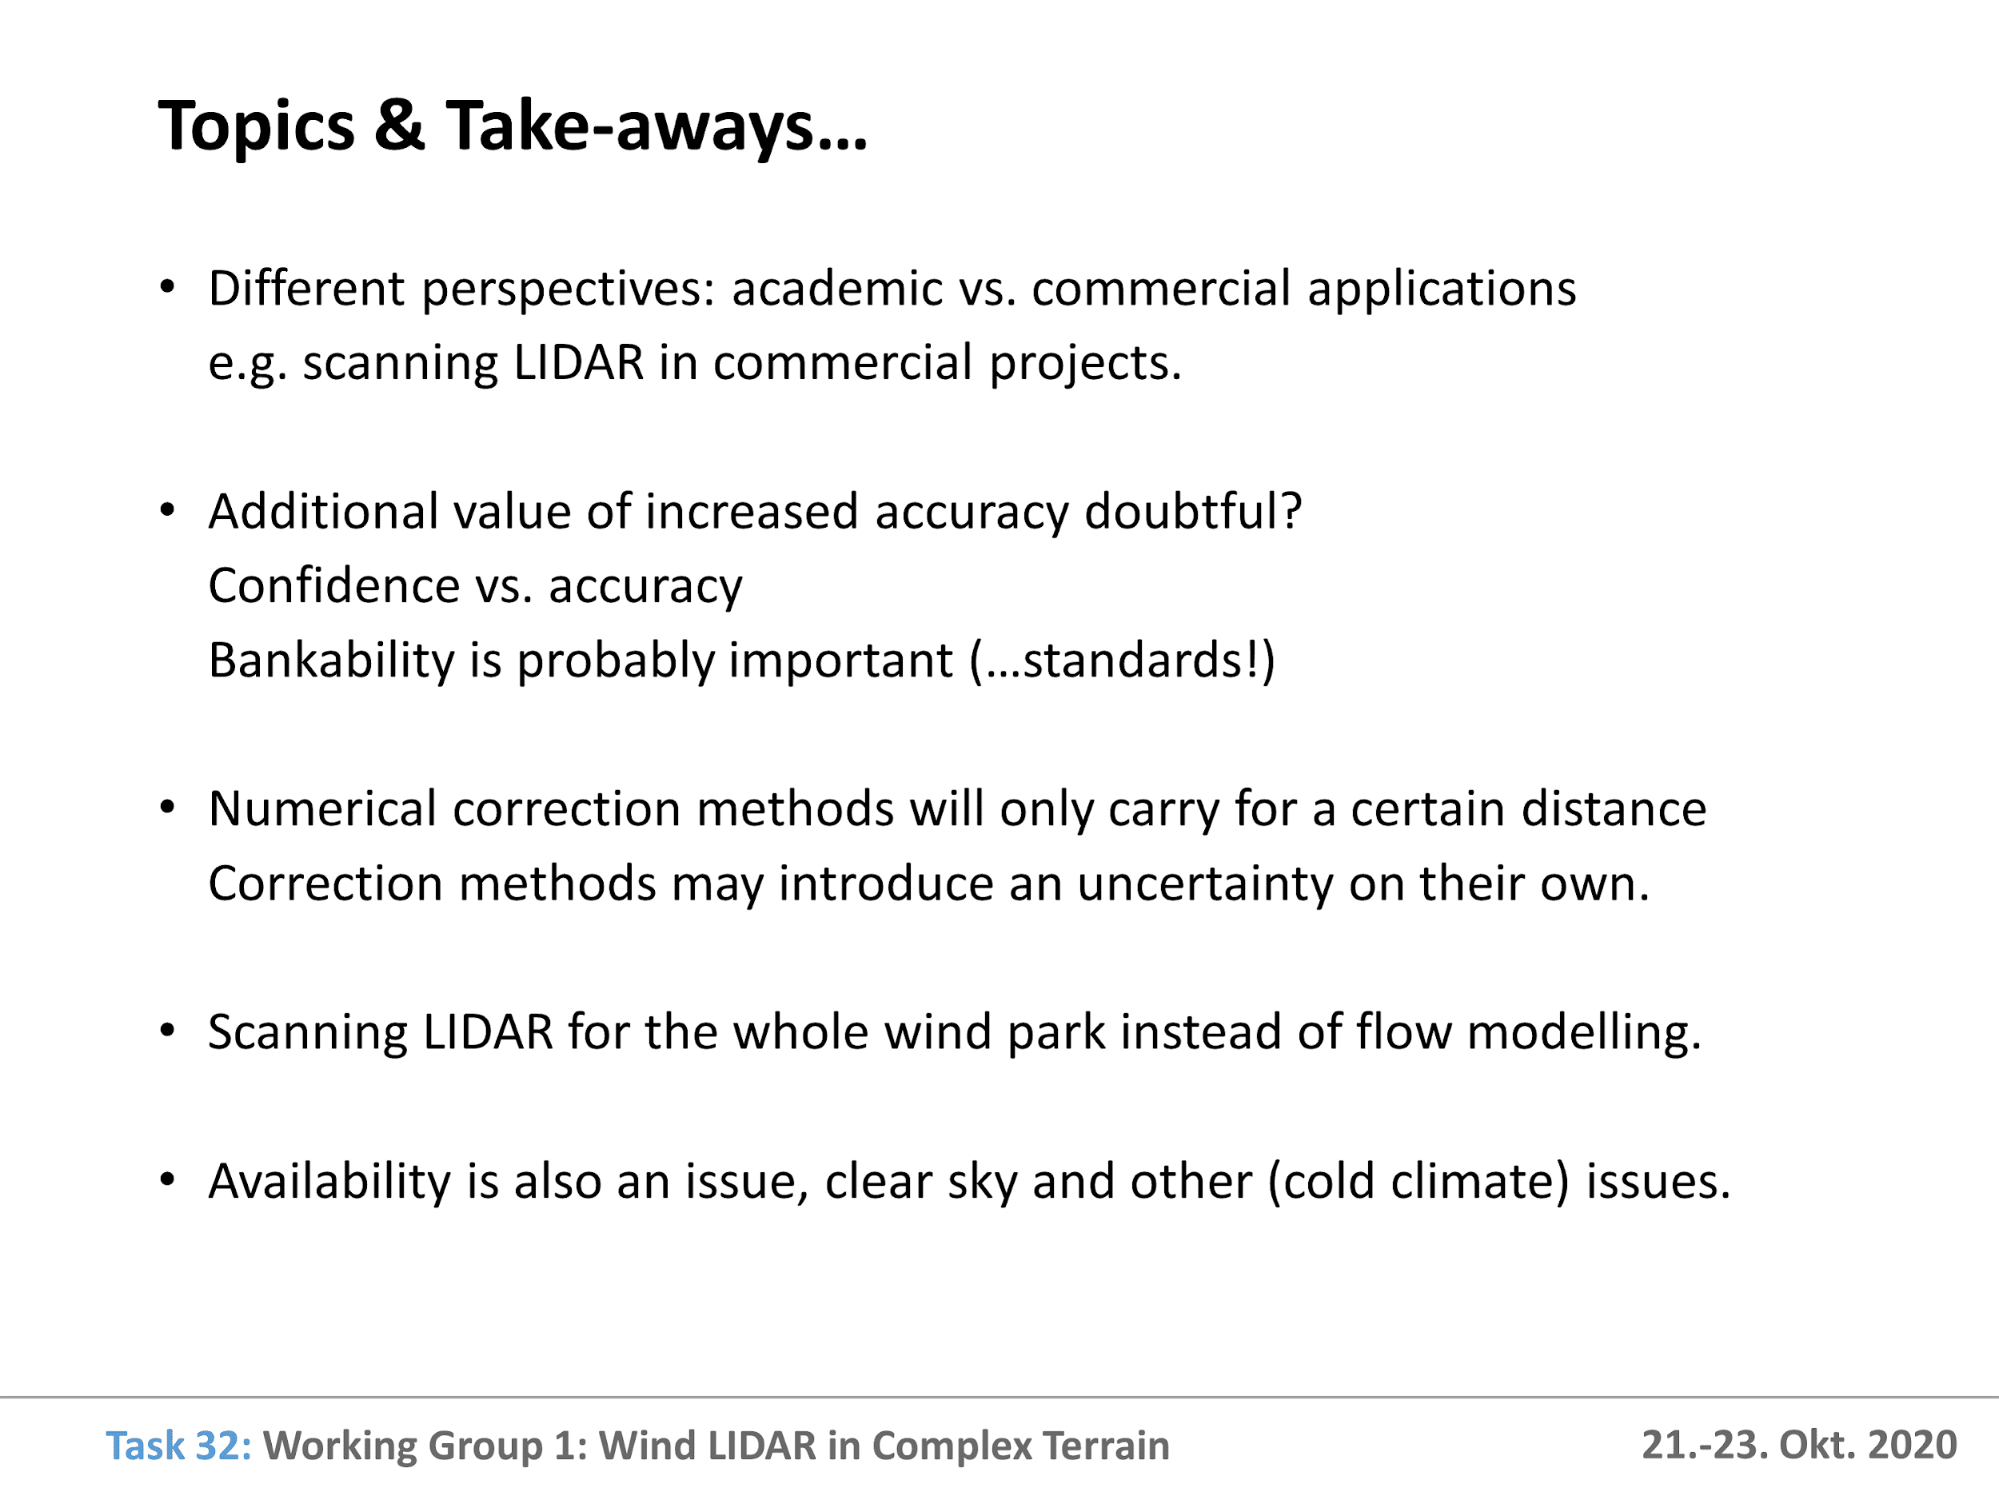
\includegraphics[width=0.85\textwidth]{figures/day3-complex-terrain.png}
%     }
%     \caption{Topics and take-aways from the complex terrain working session}
%     \label{fig:day3-complex-terrain}
% \end{figure*}

\begin{taskactions}
\textbf{Task 32 action} : Task 32 will continue to support this working
group.
\end{taskactions}

\subsubsection{Floating lidar}

\emph{Rapporteur: Julia Gottschall, IWES Fraunhofer}

The majority of actions around floating lidar are taking place through the IEC, and it is not needed at this time to have parallel activities through Task 32 as many stakeholders are already taking part in the IEC process. However, not all are involved and there is a need to make sure that the Task 32 community and IEC maintain alignment. The suggestion is therefore a third workshop in the second half of 2021 to align (\fref{fig:day3-floating-lidar}).

% \begin{figure*}[p]
%     \centering
%     \fbox{
%     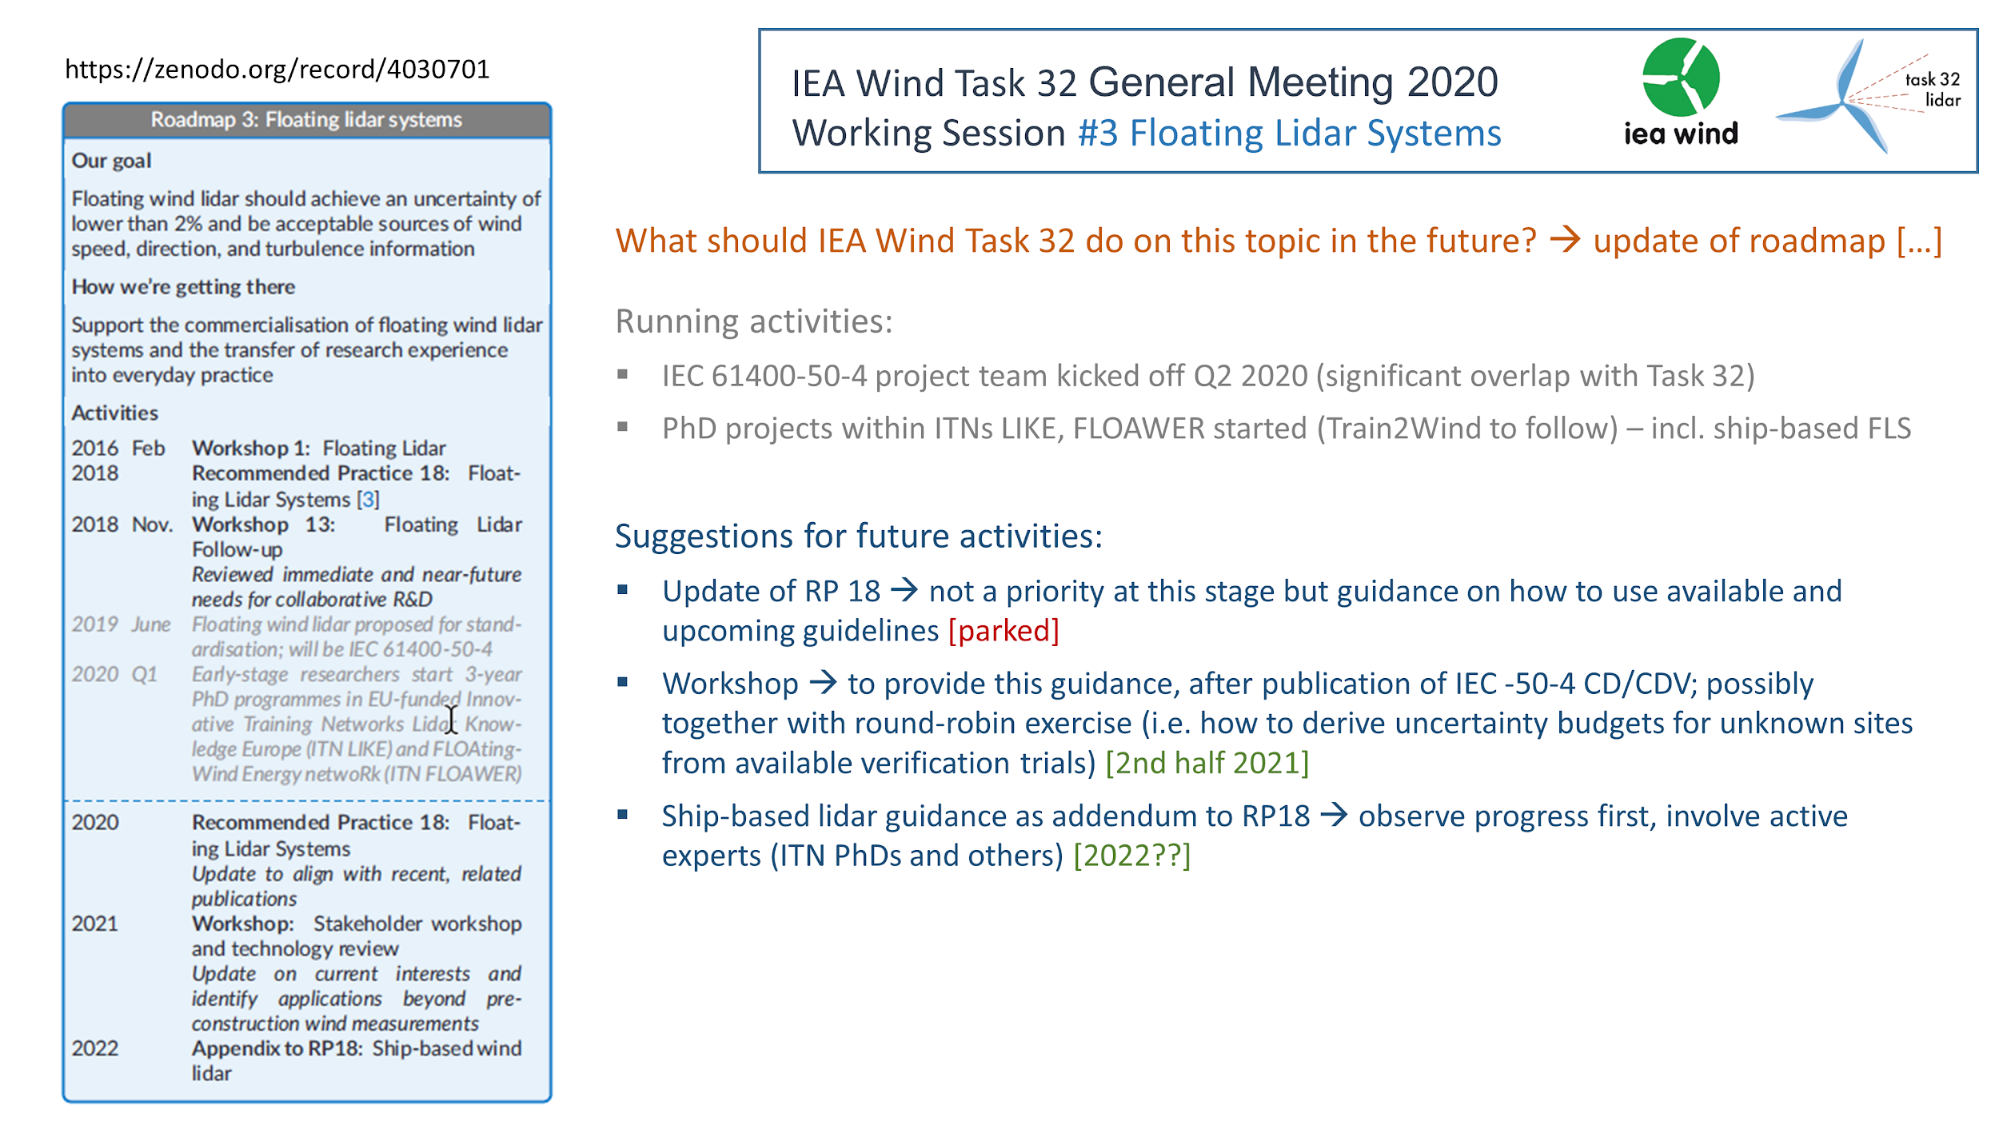
\includegraphics[width=0.85\textwidth]{figures/day3-floating-lidar.png}
%     }
%     \caption{Future activities for Task 32 around floating lidar systems.}
%     \label{fig:day3-floating-lidar}
% \end{figure*}

\begin{taskactions}
\textbf{Task 32 action}: Task 32 will organise an alignment workshop in
the second half of 2021.
\end{taskactions}

\subsubsection{Nacelle lidar in complex terrain}
\emph{Rapporteur: Jacob Burrows}

This group found that their biggest difficulty was in actually defining the problem. They produced a framework to help them and others think through the problem (\fref{fig:day3-nacelle-mounted}).

% \begin{figure*}[p]
%     \centering
%     \fbox{
%     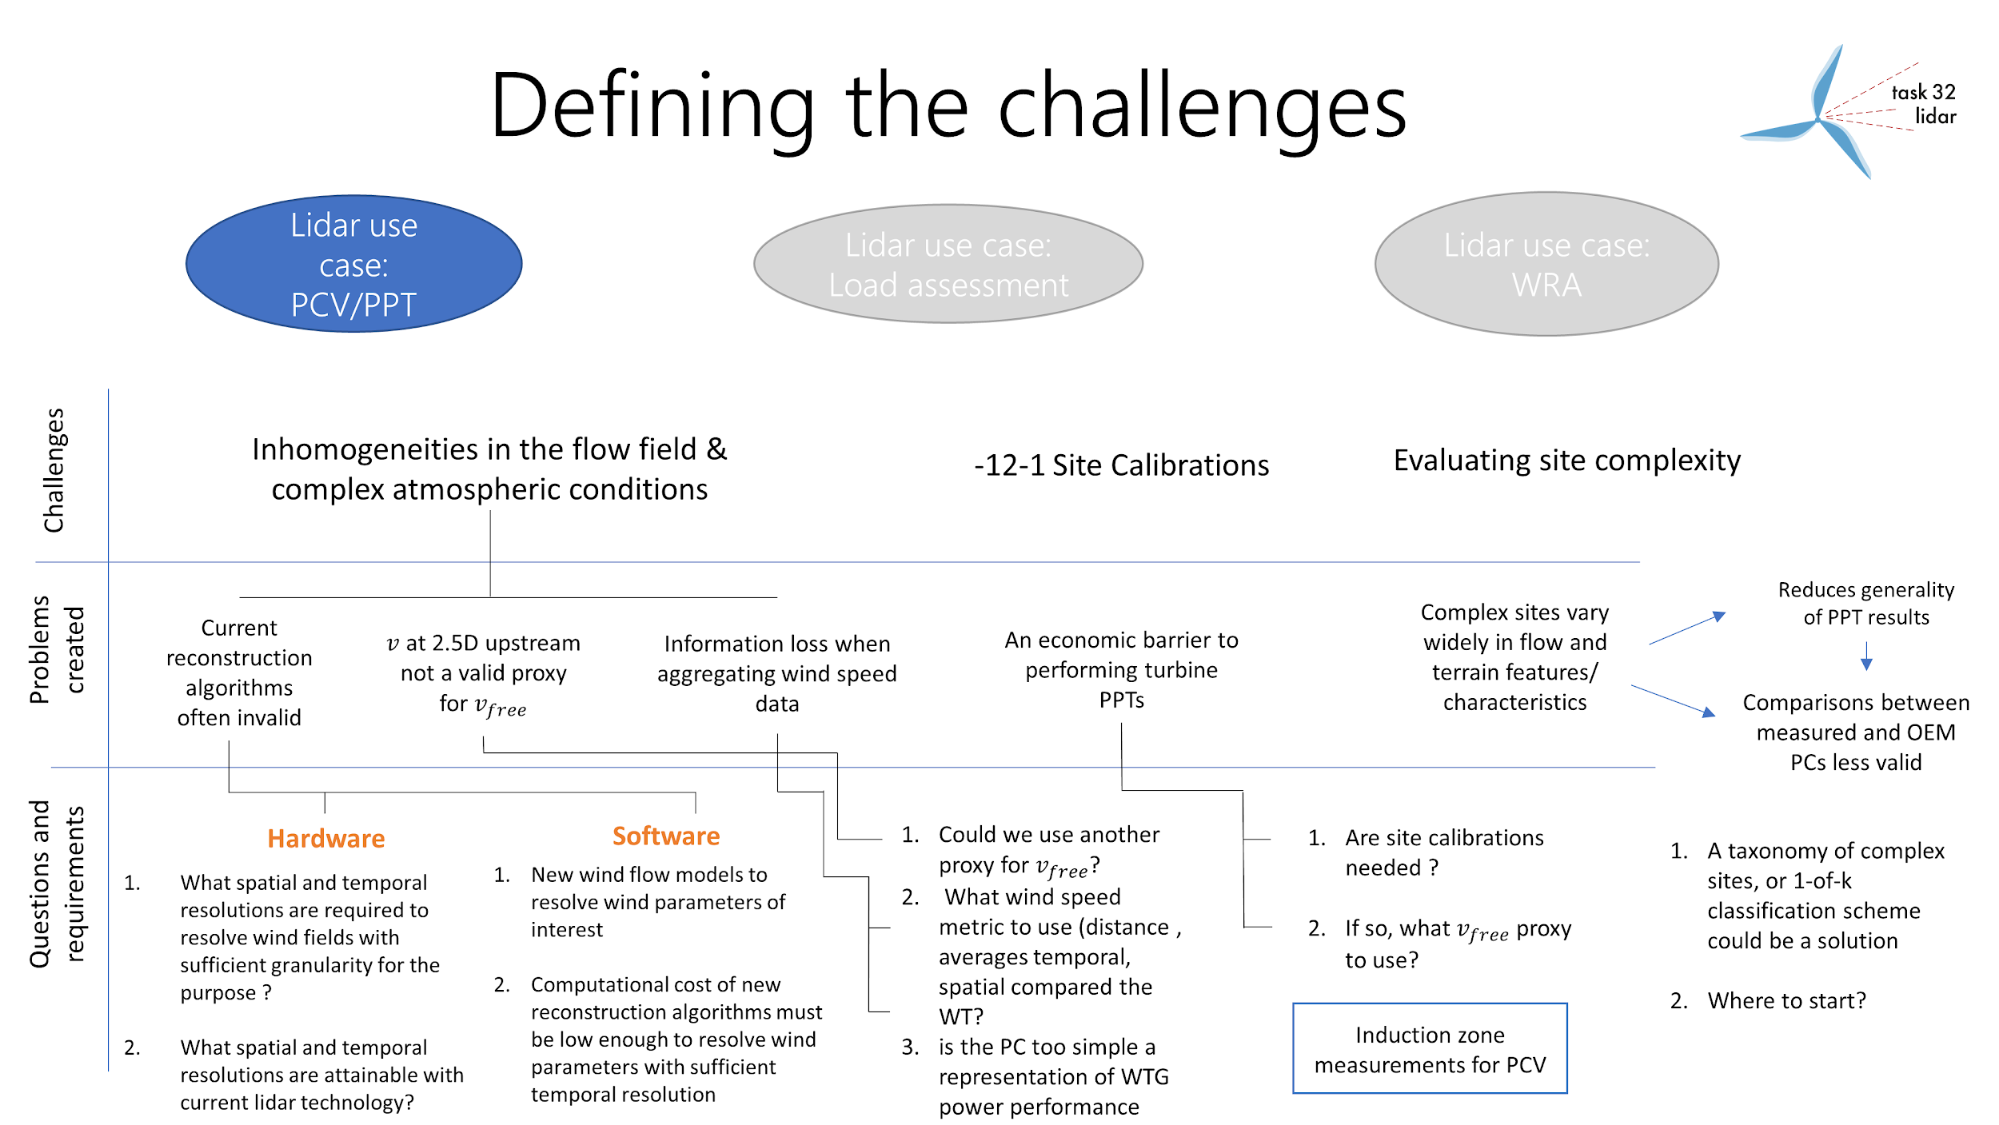
\includegraphics[width=0.85\textwidth]{figures/day3-nacelle-mounted.png}
%     }
%     \caption{Defining the challenge of using nacelle mounted lidar in complex terrain}
%     \label{fig:day3-nacelle-mounted}
% \end{figure*}

\begin{itemize}
    \item Comment from a participant: the 2.5$D$ is not a function of decay but a function of the turbine itself. Depends on the turbine size.
    \item The need is there to perform power curve verification in complex terrain from industry perspective
    \item There could be another workshop on this topic!
\end{itemize}

\begin{taskactions}
\textbf{Task 32 action}: Task 32 will combine the outcome from this group with the outcomes from the group looking at power performance verification using measurements in the induction zone. We'll also combine this with previous plans to run a round-robin on this theme. We'll propose a path forward in 2021.
\end{taskactions}

\subsubsection{Power performance verification in the induction zone}

\emph{Rapporteur: Sebastian Streitz}

The need for an alternative proxy for freestream wind speed is in common with nacelle lidar (\fref{fig:day3-powerperformance}). This suggests a need for more studies, and could also be topic for a short focused meeting.

% \begin{figure*}[p]
%     \centering
%     \fbox{
%     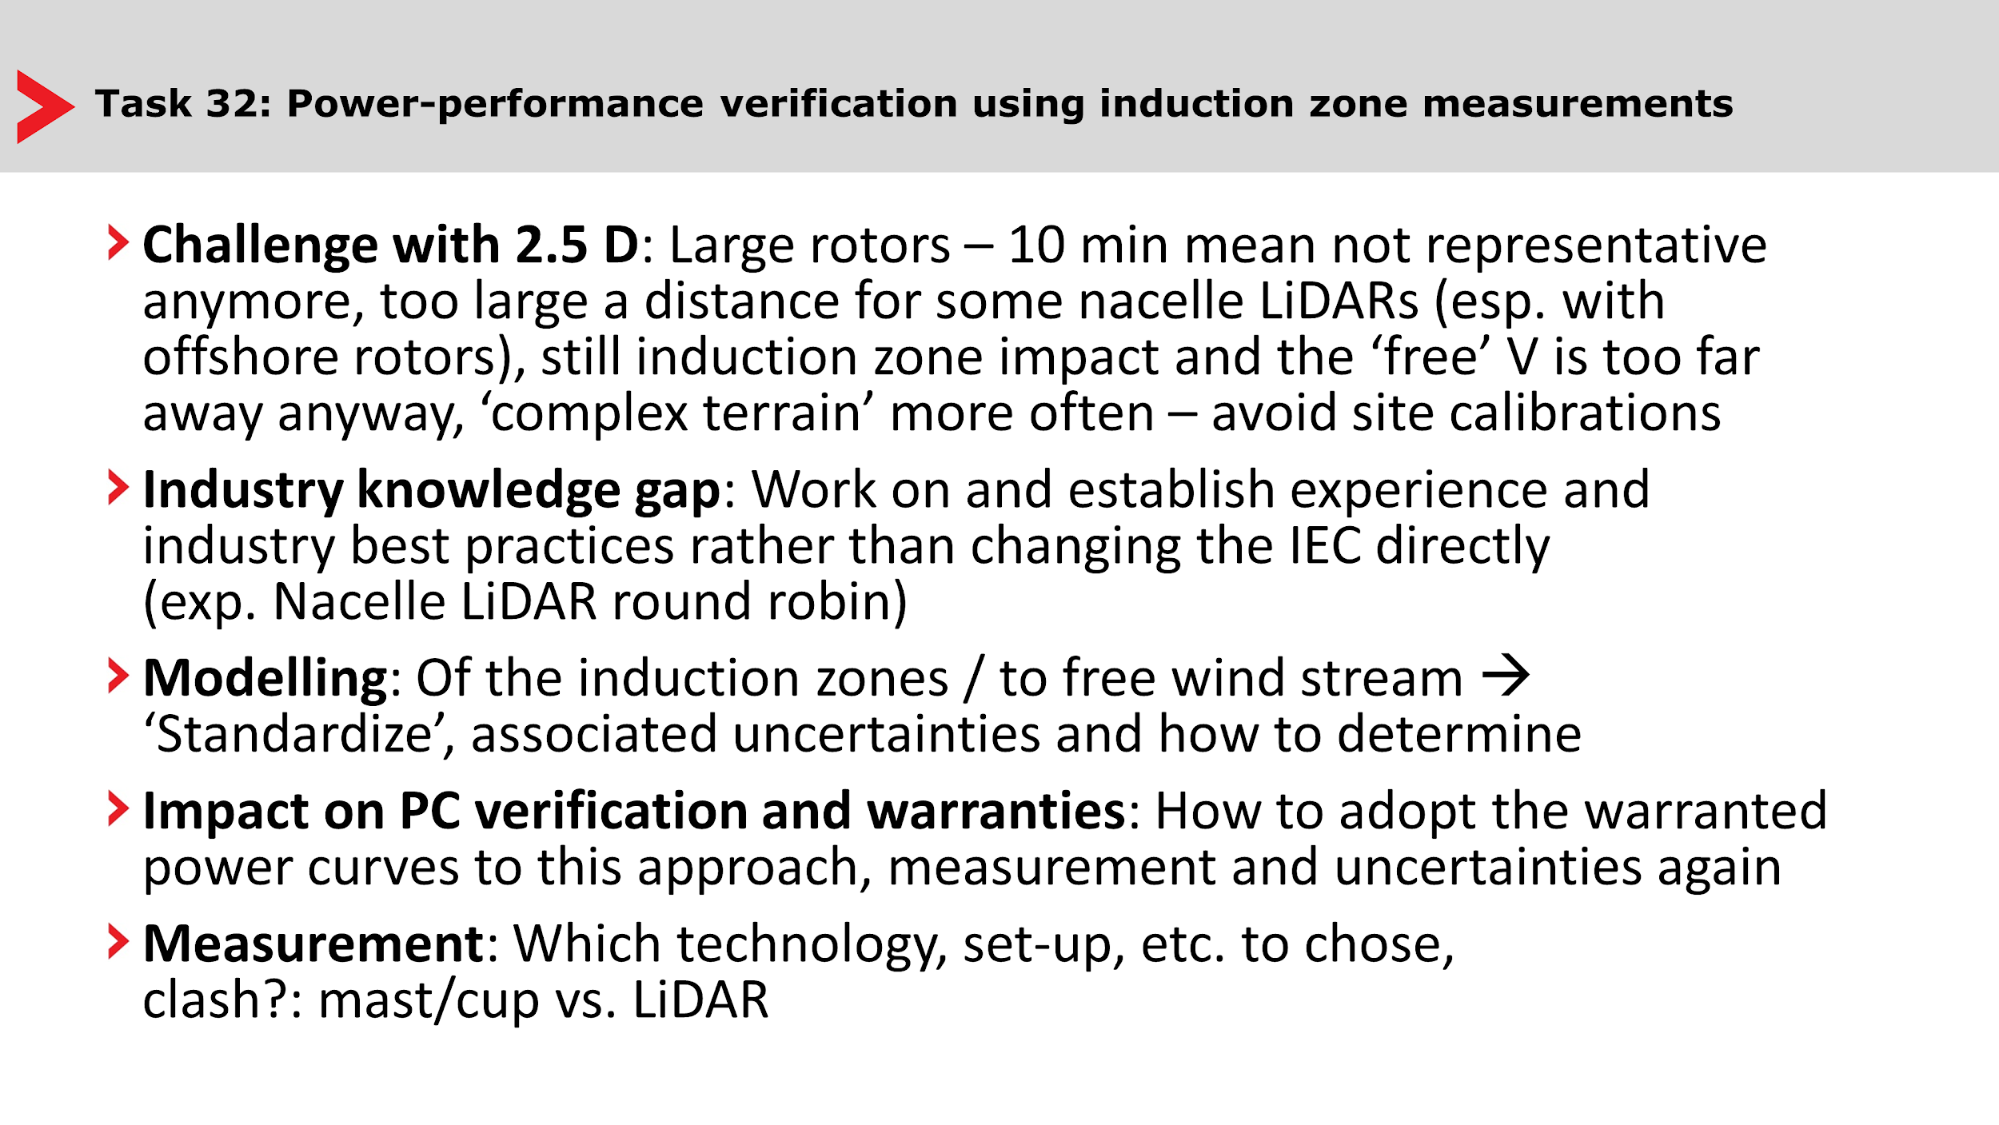
\includegraphics[width=0.85\textwidth]{figures/day3-powerperformance.png}
%     }
%     \caption{Opportunities and challenges with using measurements in the induction zone for power performance testing}
%     \label{fig:day3-powerperformance}
% \end{figure*}

\begin{taskactions}
\textbf{Task 32 action}: Task 32 will combine the outcome from this group with the outcomes from the group looking at nacelle mounted lidar in complex terrain. We'll also combine this with previous plans to run a round-robin on this theme. We'll propose a path forward in 2021.
\end{taskactions}

\subsubsection{Lidar-assisted control}

Lidar-assisted control of wind turbines is increasingly becoming reality, but turbines are not yet being designed to take full advantage of the wind lidar. There are still steps that need to be taken before co-design will become practical.

\begin{taskactions}
\textbf{Task 32 action}: Task 32 will:
\begin{enumerate}
\item Continue to work on a open repository of lidar-assisted control simulations
\item Address the cost of the lidar by a white paper: show that it has come down, improve lidar cost modeling
\item Organize a white paper to connect turbine OEM's needs to lidar manufacturers, e.g. improved availability, maintenance friendly, more adjustable
\item Collaborate more with other IEA Wind Tasks, for example Task 37 \& the new wind farm flow control Task.
\end{enumerate}
\end{taskactions}

% \begin{figure*}[p]
%     \centering
%     \fbox{
%     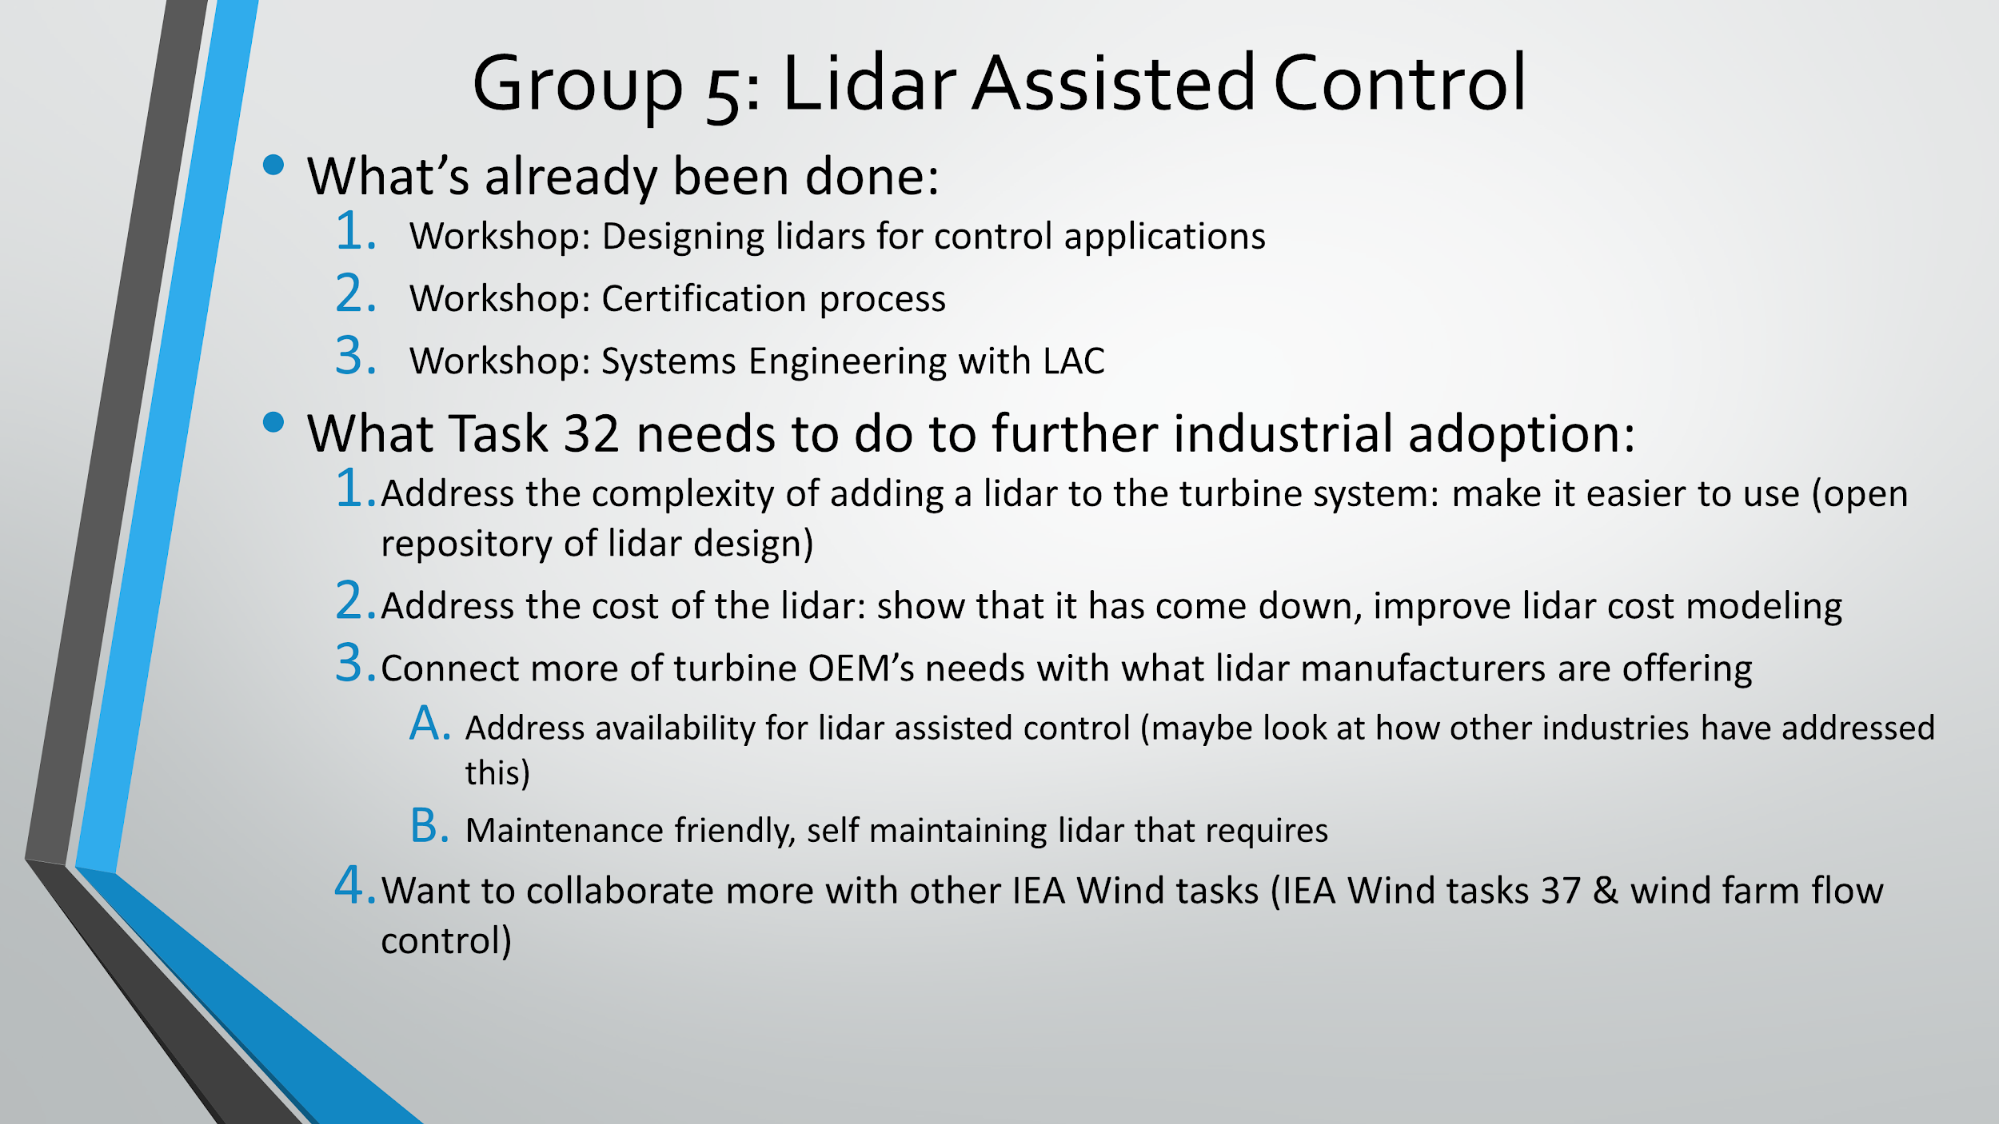
\includegraphics[width=0.85\textwidth]{figures/day3-LAC.png}
%     }
%     \caption{How Task 32 can enable adoption of lidar-assisted control of wind turbines and plants}
%     \label{fig:day3-LAC}
% \end{figure*}

The meeting closed at 17:00 CEST on 22 October.

\section{Summary}
The 2020 Task 32 General Meeting ran over three afternoons during October 2020. Three panel sessions explored the future of wind lidar technology and applications, how we might reach those goals, and how the wind lidar community might grow and change in future. Working sessions gave all members of the task the chance to catch up with current practice and cutting-edge science. And, a networking session and community news provided the opportunity for catch up with colleagues. The results from the meeting - captured in these minutes - will inform Task 32 strategy going in 2021 and beyond, and will be included in our roadmap soon \cite{clifton_2020_roadmap}. Also, the working groups that were already active in 2020 will continue into 2021 and there may be new initiatives as well.

Task 32 welcomes anyone interested in identifying and mitigating the barriers to the adoption of wind lidar. Please check \href{https://community.ieawind.org/task32/}{our website} or contact the \href{mailto:ieawind.task32@ifb.uni-stuttgart.de}{Operating Agents} to find out more.

\section{List of Participants}

The presence of a person's name or company name in this list should not be taken to imply that a person or their employer agrees with any of the opinions set out in these minutes.

% set up banded rows for the agenda and add lines to the columns
\tablehead{\rowcolor{Task32Blue2} \textbf{Name} & \textbf{Affiliation} \\ }
\arrayrulecolor{Task32Blue2!15}
\rowcolors{2}{Task32Blue2!5}{white}
\begin{supertabular}{@{}|p{0.45\columnwidth}|p{0.55\columnwidth}|@{}}
Tunahan Akbas & DTU (Student) \\
Arjun Anantharaman & University of Oldenburg \\
Oliver Bischoff & SWE, U. Stuttgart \\
 Jacob Burrows & EDF \\
 Steven Clark & NRG Systems \\
 Andy Clifton & SWE, U. Stuttgart \\
 Peter Clive & Black and Veatch \\
 Francisco Costa & SWE, U. Stuttgart \\
 Andrew Davidson & sse renewables \\
 Reesa Dexter & DNV GL \\
 Rémi Gandoin & C2Wind \\
 Ashim Giyanani & Fraunhofer IWES \\
 Julia Gottschall & Fraunhofer IWES \\
 Fabrice Guillemin & IFPEN \\
 Feng Guo & DTU Wind Energy \\
 Thom Homsma & Siemens Gamesa Renewable Energy \\
 Yasmin Hubmann & OX2\\
 Poul Hummelshøj & METEK Nordic ApS \\
 Masaharu Imaki & Mitsubishi Electric Corporation \\
 Hans Jørgensen & DTU Wind Energy \\
 Senthilnathan K & \\
 Velmurugan Karuppiah & \\
 Aidan Keane & Wood Renewables \\
 Felix Kelberlau & Fugro \\
 Sara Koller & Meteotest \\
 Gyeongil Kwak & Engie \\
 Wiebke Langreder & EMD International A/S \\
 Christophe Lepaysan & EPSILINE \\
 Dexing Liu & SWE, U. Stuttgart \\
 Alvaro Matesanz & Vestas \\
 Rhys Neild & DNV GL \\
 Arthur Ostyn & 3E \\
 Alkistis Papetta & Fraunhofer IWES \\
 Mariìa Joseì Pedrayes & Vestas \\
 Mihajlo Raljic &  \\
 Jens Riechert & DNV GL \\
 Rebeca Rivera Lamata & DTU Wind Energy \\
 Peter Rosenbusch & Leosphere \\
 Hugo Rubio & Fraunhofer IWES \\
 Mads Sørensen & EMD International A/S \\
 Pedro Santos & DTU Wind Energy \\
 Okan Sargin & Guidehouse WTTS \\
 David Schlipf & Flensburg University of Applied Sciences \\
 Carolin Schmitt & EnBW \\
 Andrew Scholbrock & National Renewable Energy Laboratory \\
 Eric Simley & National Renewable Energy Laboratory \\
 Elliot Simon & DTU Wind Energy \\
 Chris Slinger & ZX Lidars \\
 Alexander Stoekl & Energiewerkstatt \\
 Sebastian Streitz & Nordex Group \\
 Davide Trabucchi & Deutsche Windguard Consulting \\
 Vasilis Vasileiadis & \\
 Anish Venu & DNV GL \\
 Jochem Vermeir & Tractebel Engie \\
 Marcel Weber & Enercon \\
 Ellie Weyer & UL \\
 Gerrit Wolken-Möhlmann & Fraunhofer IWES \\
 Alex Woodward & ZX Lidars \\
 Ines Wuerth & SWE, U. Stuttgart \\
\end{supertabular}
 
\section{Acknowledgements}
The meeting was moderated by Andrew (Andy) Clifton, Task 32 Operating Agent. The working group sessions were facilitated by David Schlipf, Task 32 Operating Agent, many members of the Task 32 Advisory Board, and members of the Task 32 community. The minutes were written by Ines Würth and David Schlipf and then converted into this document by Andrew Clifton.


%% -----------------------------------
%% References
%% -----------------------------------
%\section*{References}
% bibliography
\label{sec:References}
\addcontentsline{toc}{section}{References}
{\small
	\printbibliography
}
\vspace*{\fill}

%% -----------------------------------
%% Outlined block of smaller text
%% -----------------------------------
\begin{tcolorbox}[width=1.0\columnwidth,
		boxsep=0pt,
		left=3pt,
		right=3pt,
		top=3pt,
		arc=0pt,
		boxrule=0.5pt,
		toprule=0.5pt,
		colback=white,
		coltext=TextGrey
	]
	{\footnotesize

		%% -----------------------------------
		%% IEA WIND AND TASK 32
		%% -----------------------------------
		
		\begin{tabular}{m{0.3\columnwidth}m{0.6\columnwidth}}
			\rowcolor{white}
			\multicolumn{2}{p{0.9\columnwidth}}{%
			This document was self published by IEA Wind Task 32.
			}\\
			% IEA Wind * DO NOT EDIT THIS TEXT *
			\rowcolor{white}
			
\includegraphics[height=2cm]{graphics/IEAWind_logo.jpg}  &
			The International Energy Agency is an autonomous organisation which works to ensure reliable, affordable and clean energy for its 30 member countries and beyond. The IEA Wind Technology Collaboration Programme supports the work of 38 independent, international groups of experts that enable governments and industries from around the world to lead programmes and projects on a wide range of energy technologies and related issues.%
			\\
			% Task 32 * DO NOT EDIT THIS TEXT *
			\rowcolor{white}
			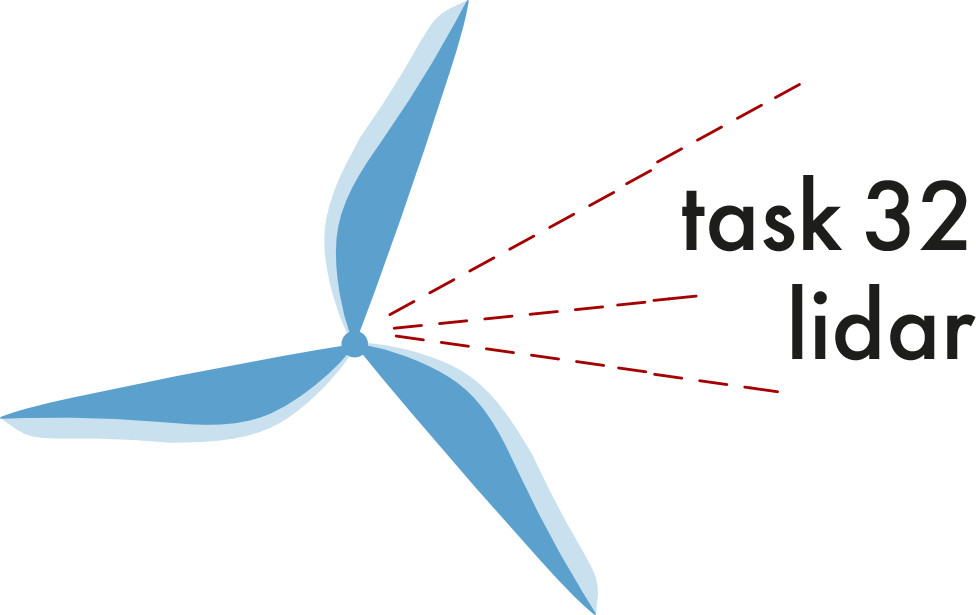
\includegraphics[height=1.5cm]{graphics/Task32_logo.jpg} &
			\href{https://community.ieawind.org/task32/home}{IEA Wind Task 32} exists to identify and mitigate the barriers to the deployment of wind lidar for wind energy applications.\\
			% authors, etc
			\rowcolor{white}
			\multicolumn{2}{p{0.9\columnwidth+2\tabcolsep}}{%
		%% -----------------------------------
		%% For more information
		%% -----------------------------------
		% N.B. do not add line breaks between the next items
		\textbf{For more information:} See the  \href{https://community.ieawind.org/task32/home}{Task 32 website}.
		%% -----------------------------------
		%% Authors
		%% -----------------------------------
		\textbf{Author team:} %
		Andrew Clifton (Task 32 Operating Agent, University of Stuttgart, Germany), %
		Ines Würth (SWE, University of Stuttgart, Germany), %		
		David Schlipf (Task 32 operating Agent, Flensburg University of Applied Sciences, Germany).
		%% -----------------------------------
		%% Reviewers
		%% -----------------------------------
		%\textbf{Reviewers:} %
		% first last (short affiliation), %
		% first last (short affiliation).
		%% -----------------------------------
		%% Images
		%% -----------------------------------
		\textbf{Images:}
		Banner, left to right: \href{https://unsplash.com/@alexkixa}{Alexandre Debiève on Unsplash}, \href{http://ifb.uni-stuttgart.de}{SWE U. Stuttgart}, \href{https://unsplash.com/@markusspiske}{Markus Spiske on Unsplash}.
	}\\
	\end{tabular}%

	}

	%% -----------------------------------
	%% End of highlighted block
	%% -----------------------------------
\end{tcolorbox}
\vspace*{\fill}

\newpage
%\subsection{Summary slides from the working sessions}

\begin{figure*}[p]
    \centering
    \fbox{
    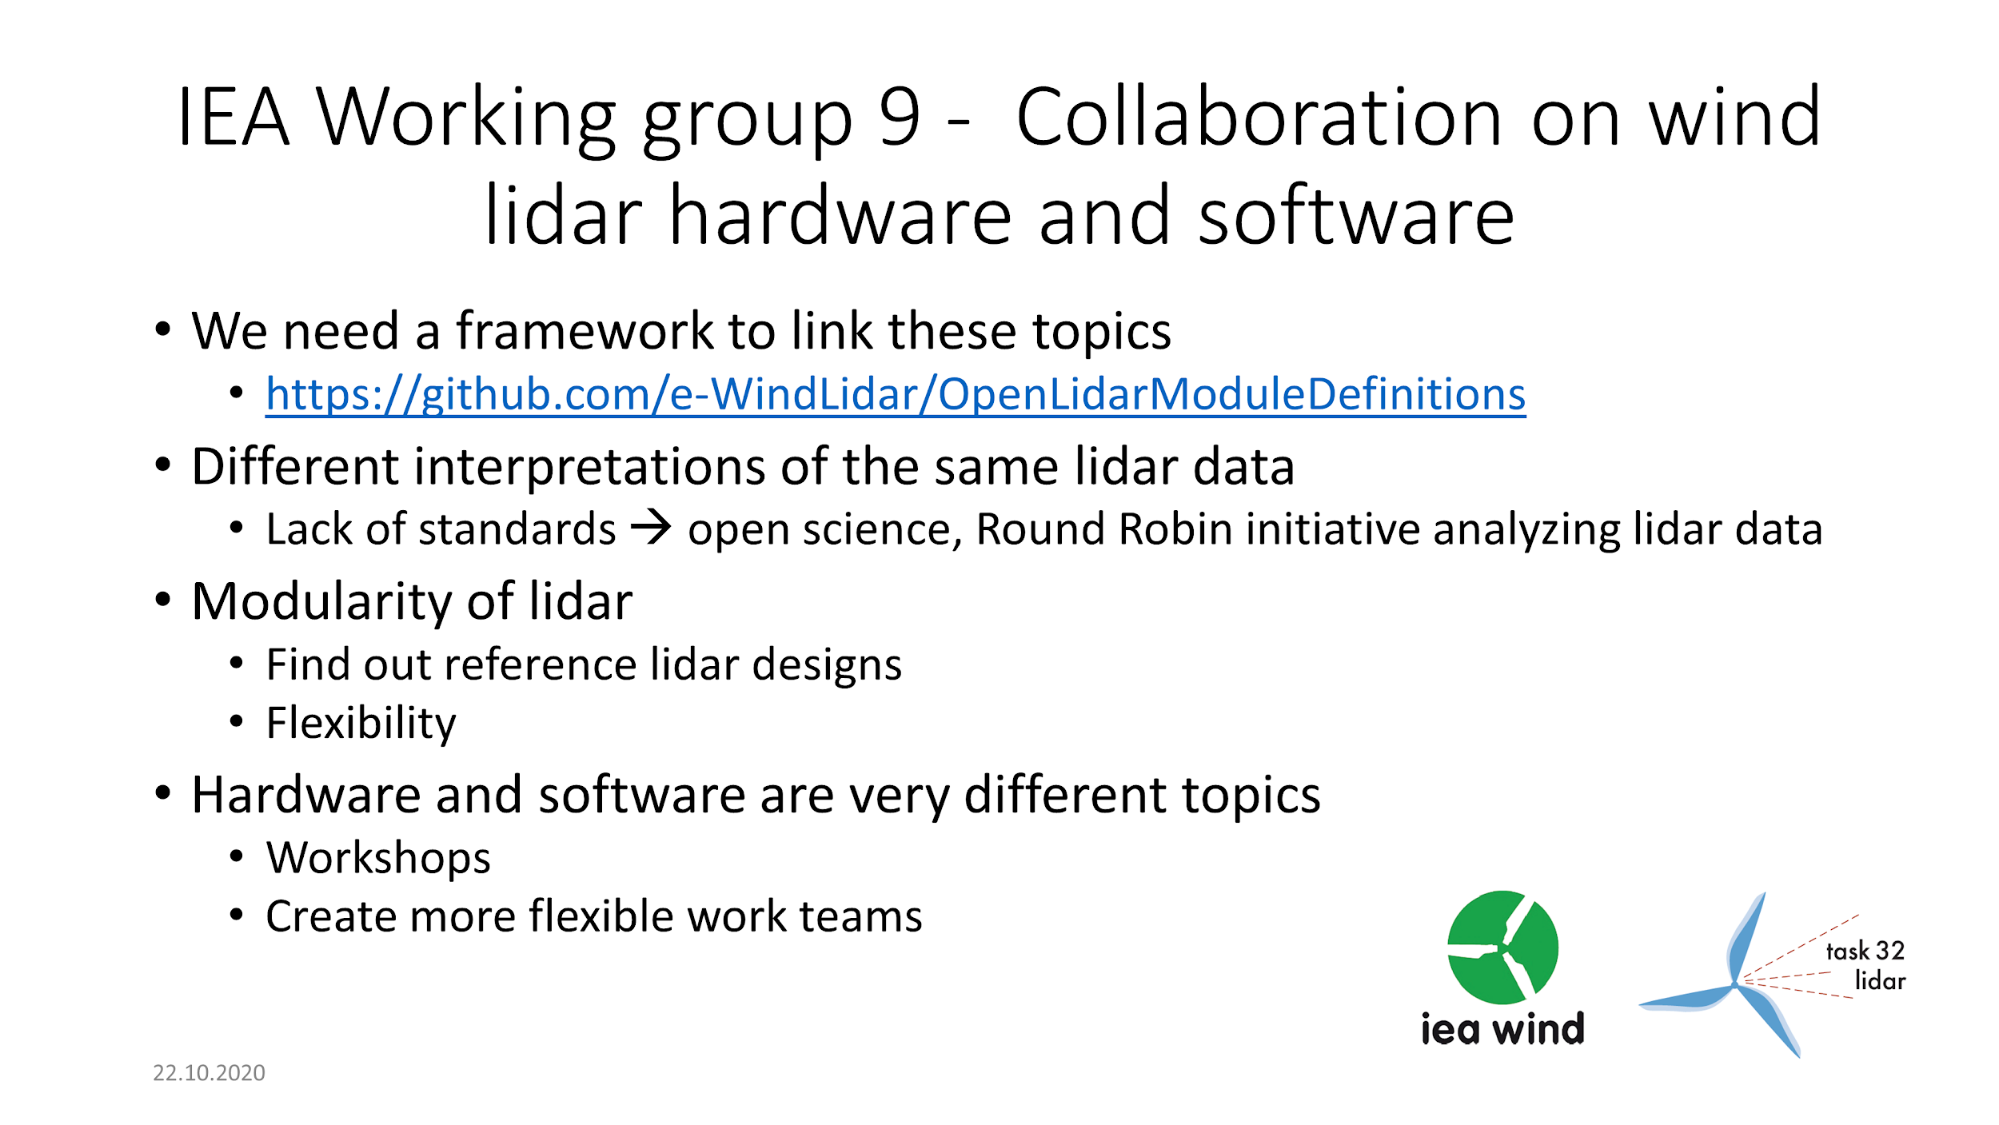
\includegraphics[width=0.85\textwidth]{figures/day3-collaboration-hardware-software.png}
    }
    \caption{Collaboration on wind lidar hardware and software}
    \label{fig:day3-collaboration-hardware-software}
\end{figure*}

\begin{figure*}[p]
    \centering
    \fbox{
    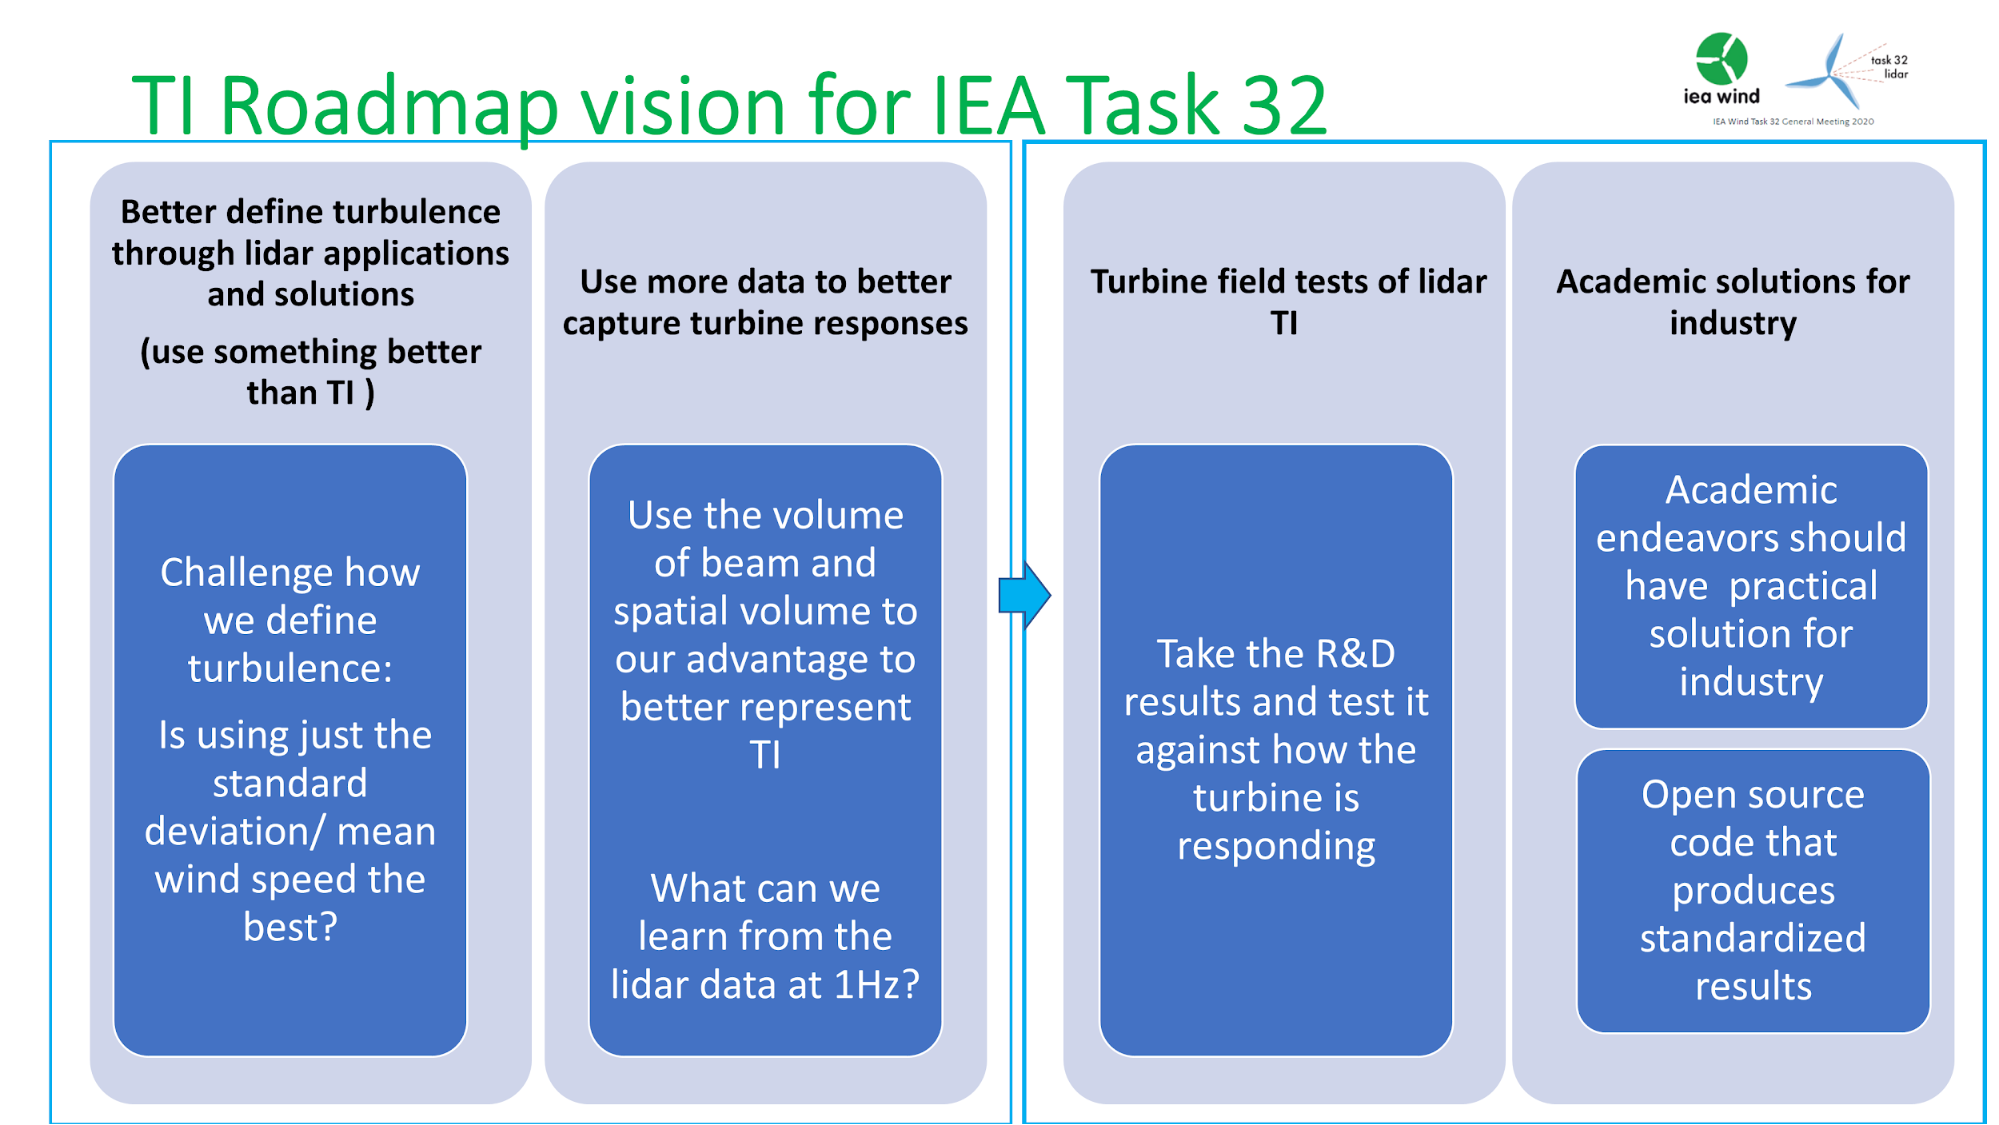
\includegraphics[width=0.85\textwidth]{figures/day3-Ti-group.png}
    }
    \caption{A lidar-derived turbulence data roadmap vision for Task 32 }
    \label{fig:day3-Ti-group}
\end{figure*}

\begin{figure*}[p]
    \centering
    \fbox{
    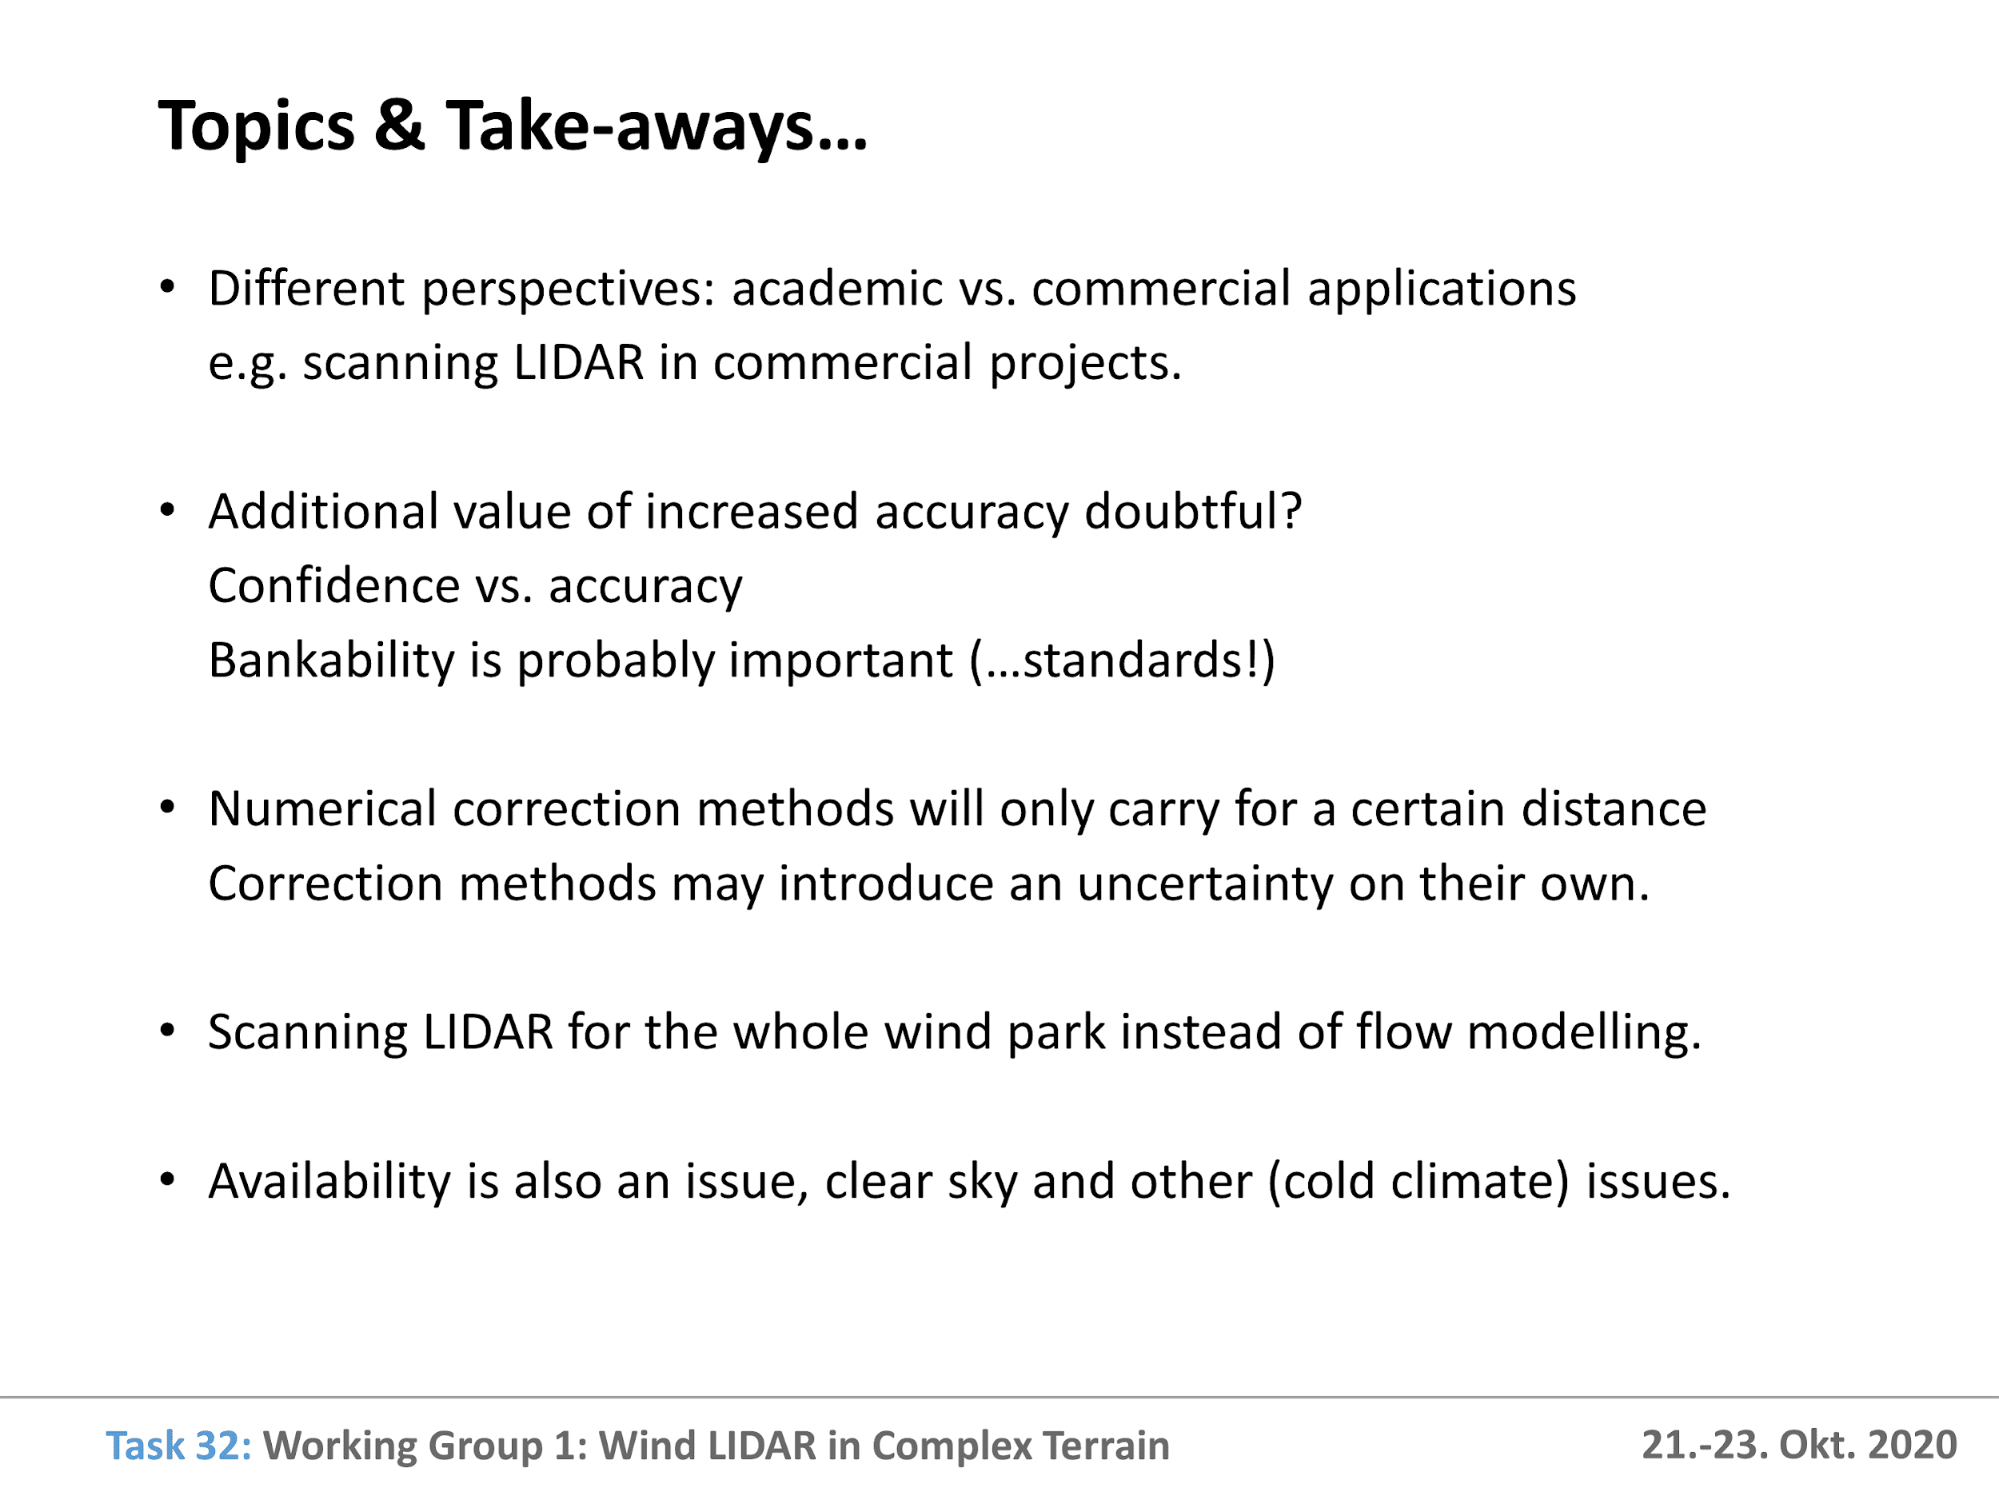
\includegraphics[width=0.85\textwidth]{figures/day3-complex-terrain.png}
    }
    \caption{Topics and take-aways from the complex terrain working session}
    \label{fig:day3-complex-terrain}
\end{figure*}

\begin{figure*}[p]
    \centering
    \fbox{
    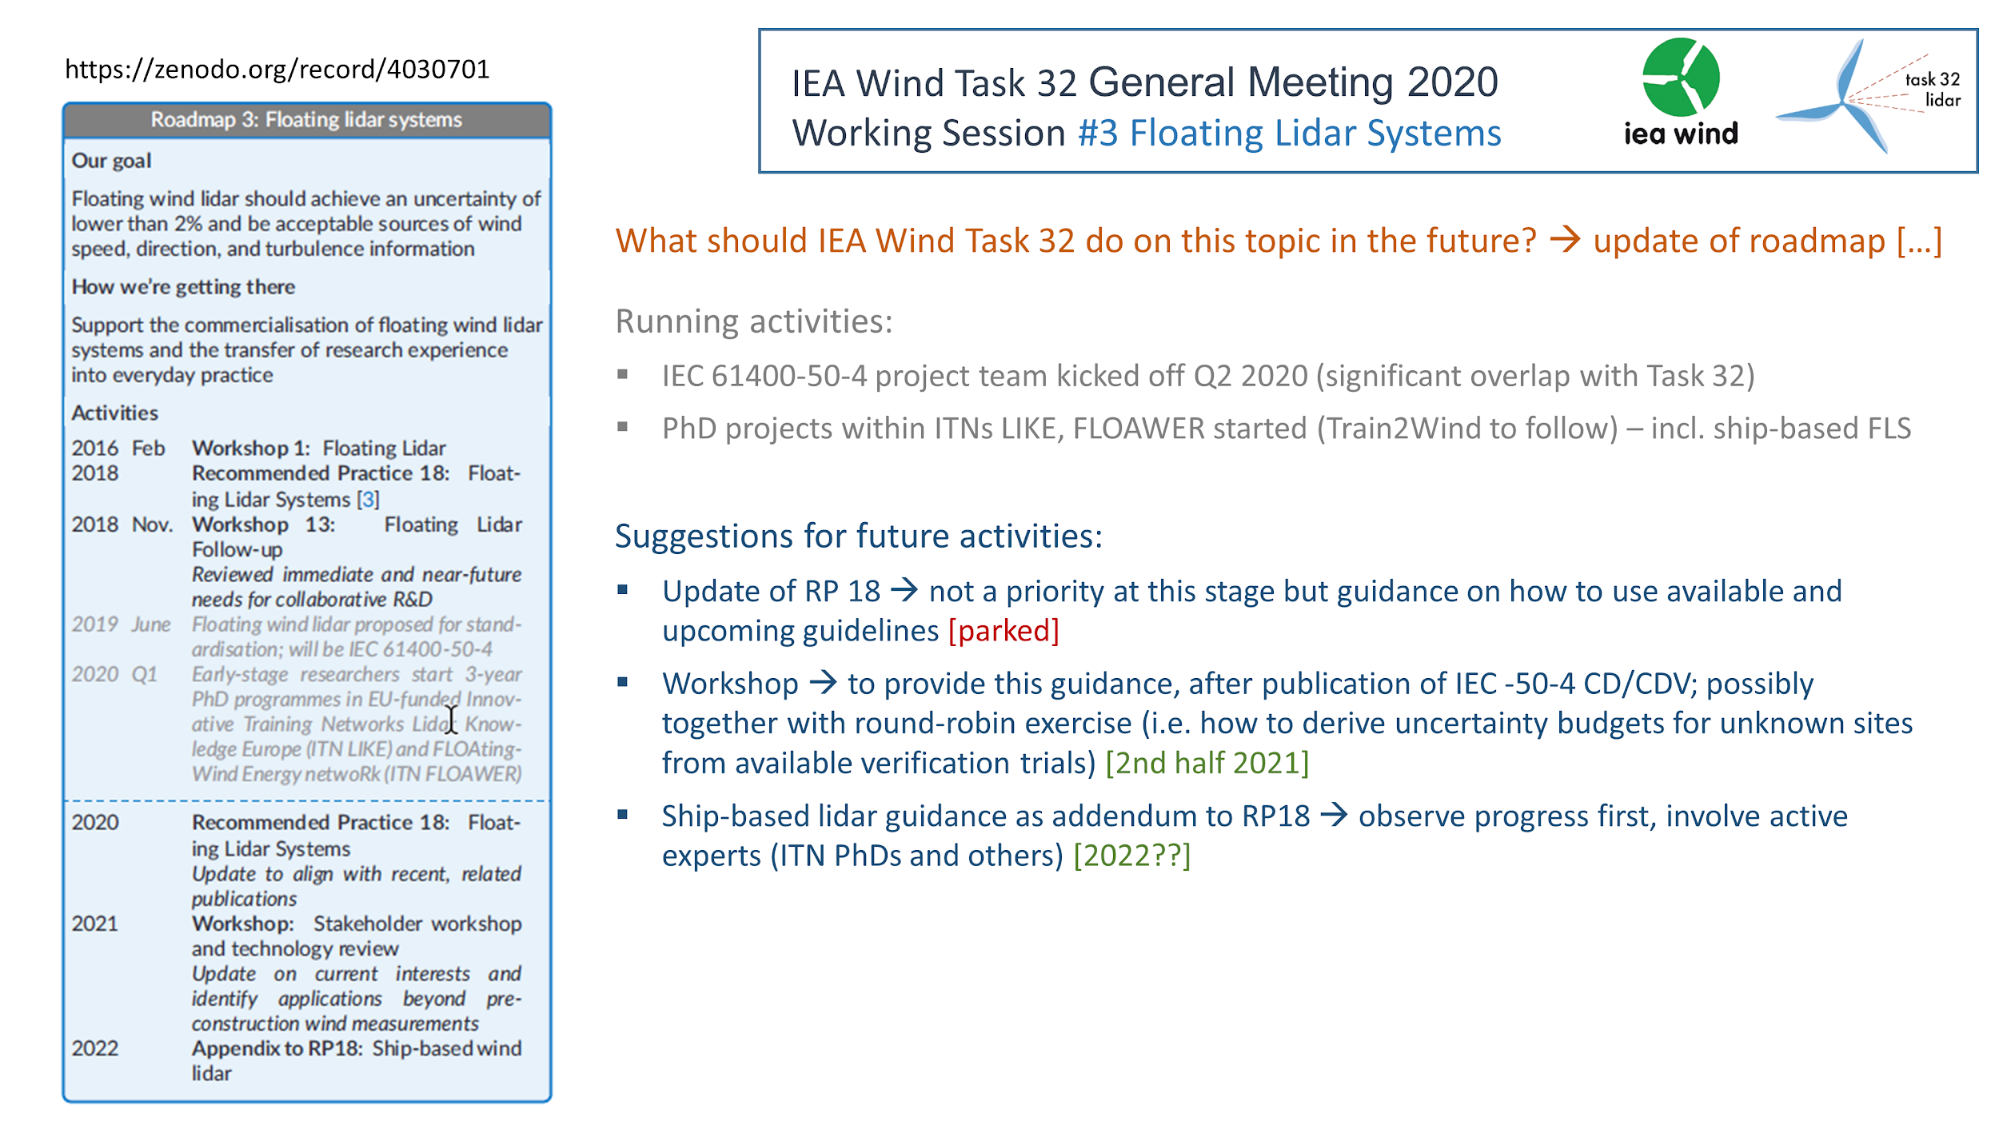
\includegraphics[width=0.85\textwidth]{figures/day3-floating-lidar.png}
    }
    \caption{Future activities for Task 32 around floating lidar systems.}
    \label{fig:day3-floating-lidar}
\end{figure*}

\begin{figure*}[p]
    \centering
    \fbox{
    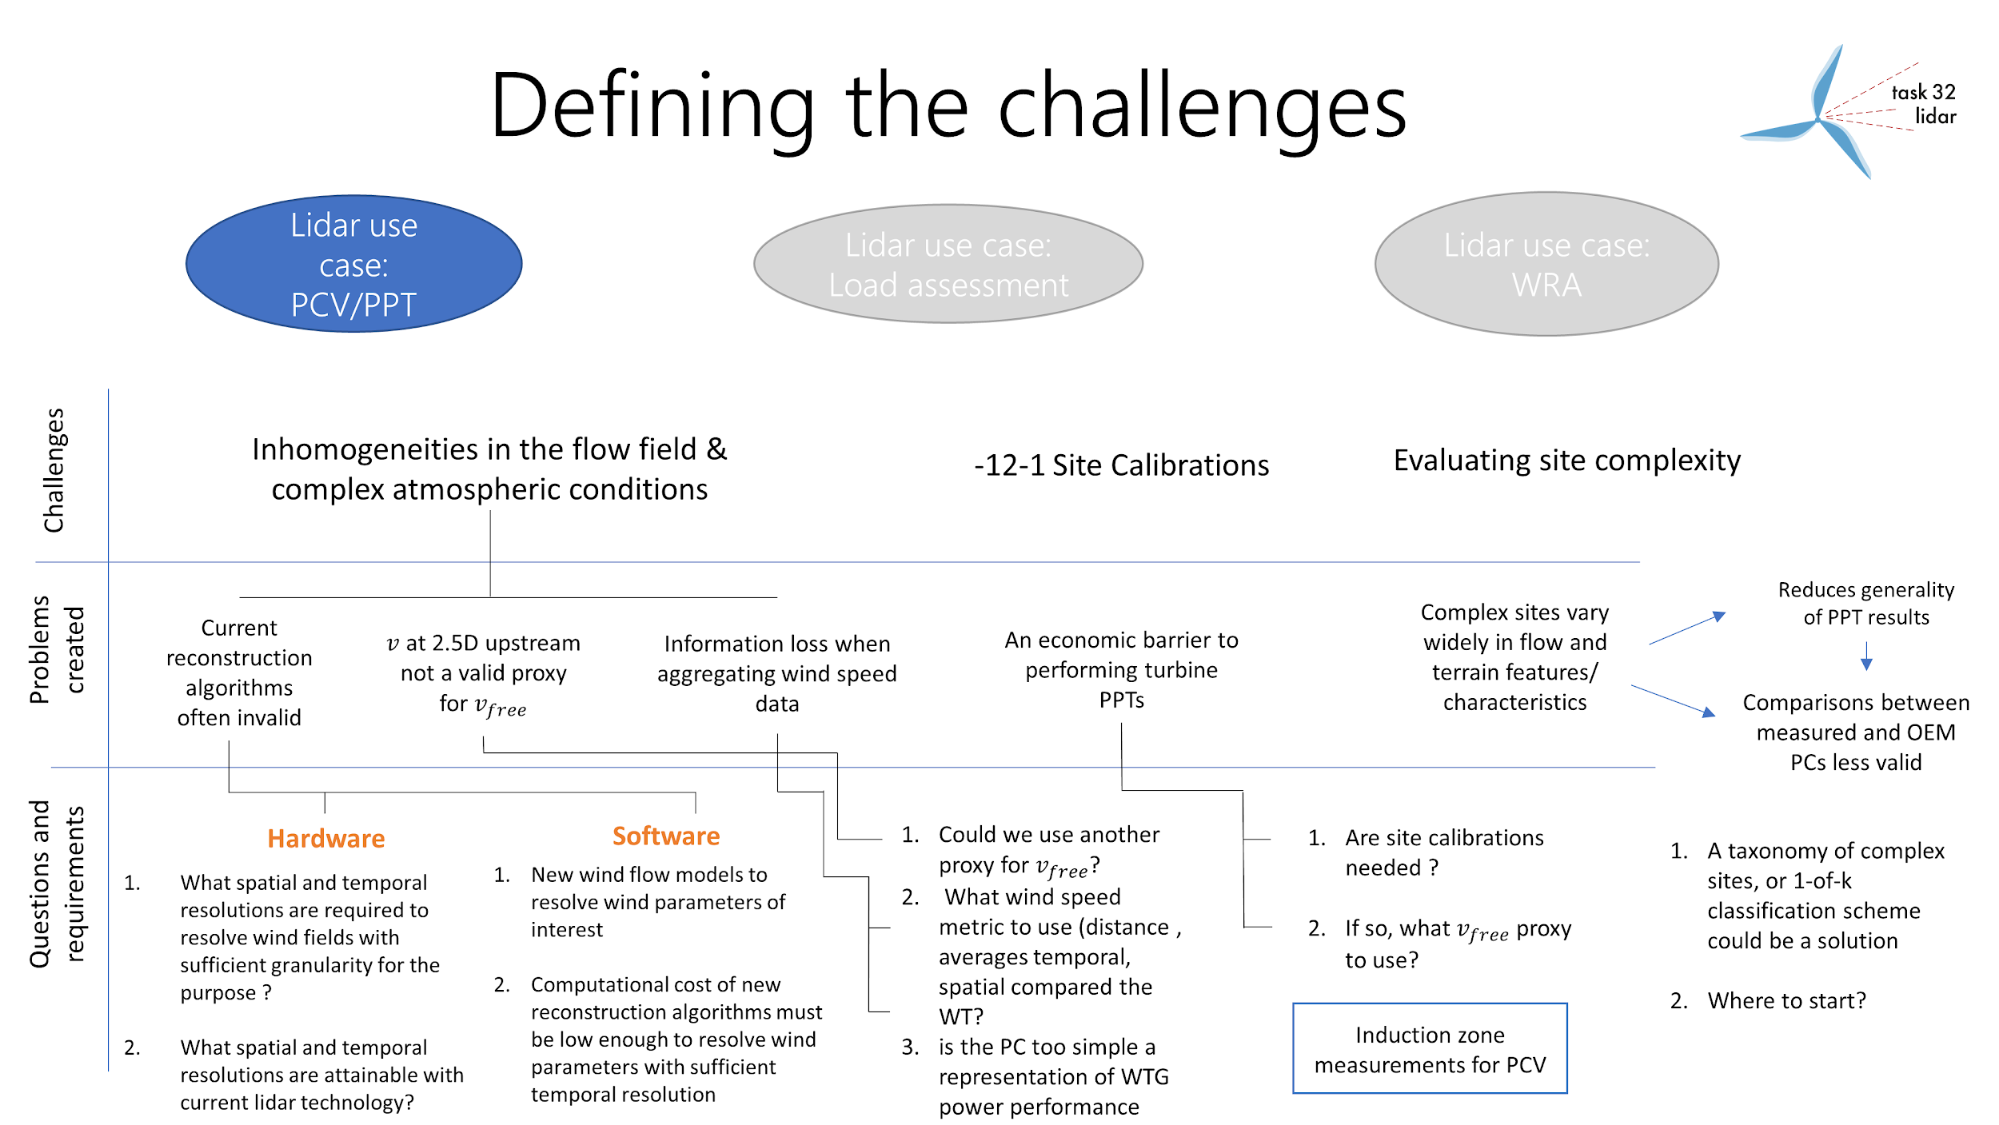
\includegraphics[width=0.85\textwidth]{figures/day3-nacelle-mounted.png}
    }
    \caption{Defining the challenge of using nacelle mounted lidar in complex terrain}
    \label{fig:day3-nacelle-mounted}
\end{figure*}

\begin{figure*}[p]
    \centering
    \fbox{
    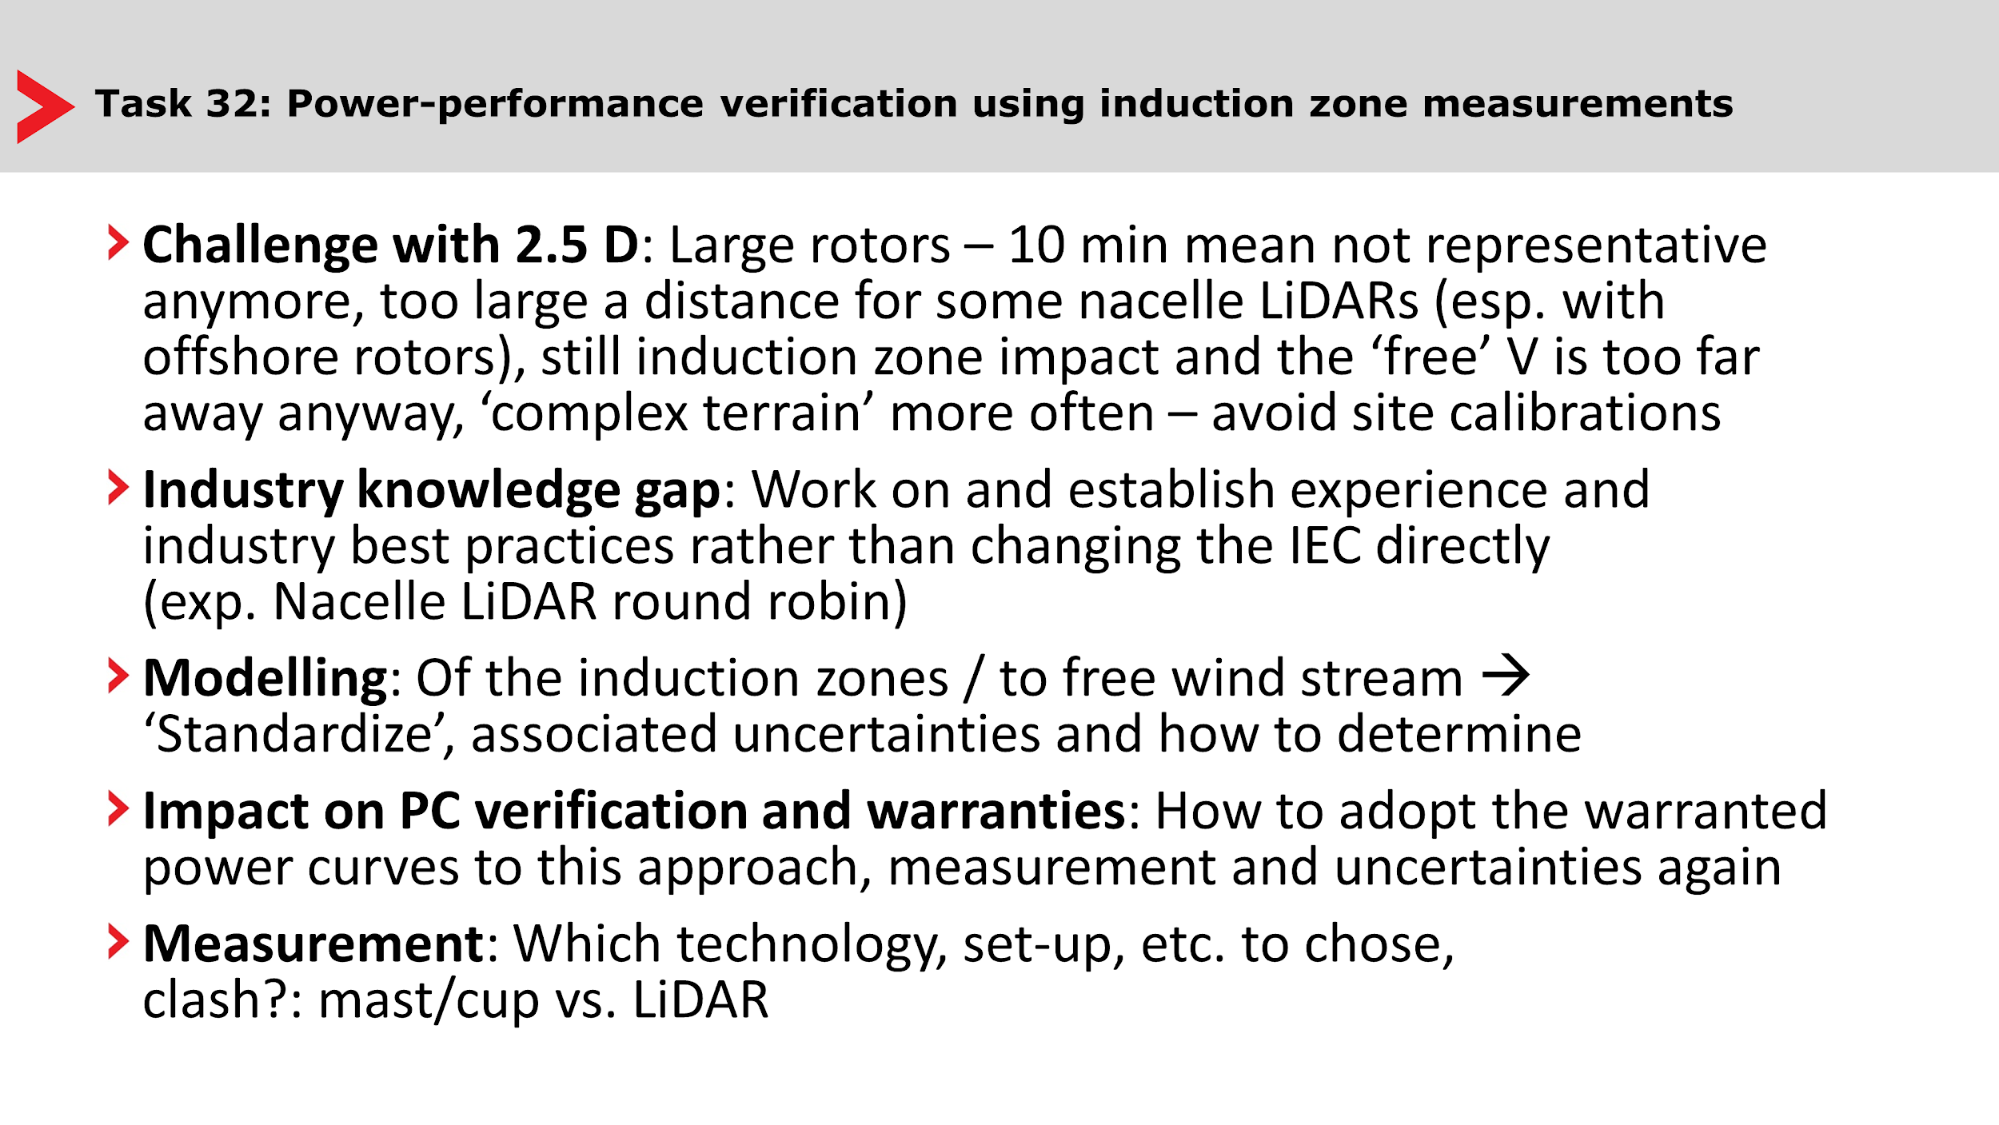
\includegraphics[width=0.85\textwidth]{figures/day3-powerperformance.png}
    }
    \caption{Opportunities and challenges with using measurements in the induction zone for power performance testing}
    \label{fig:day3-powerperformance}
\end{figure*}

\begin{figure*}[p]
    \centering
    \fbox{
    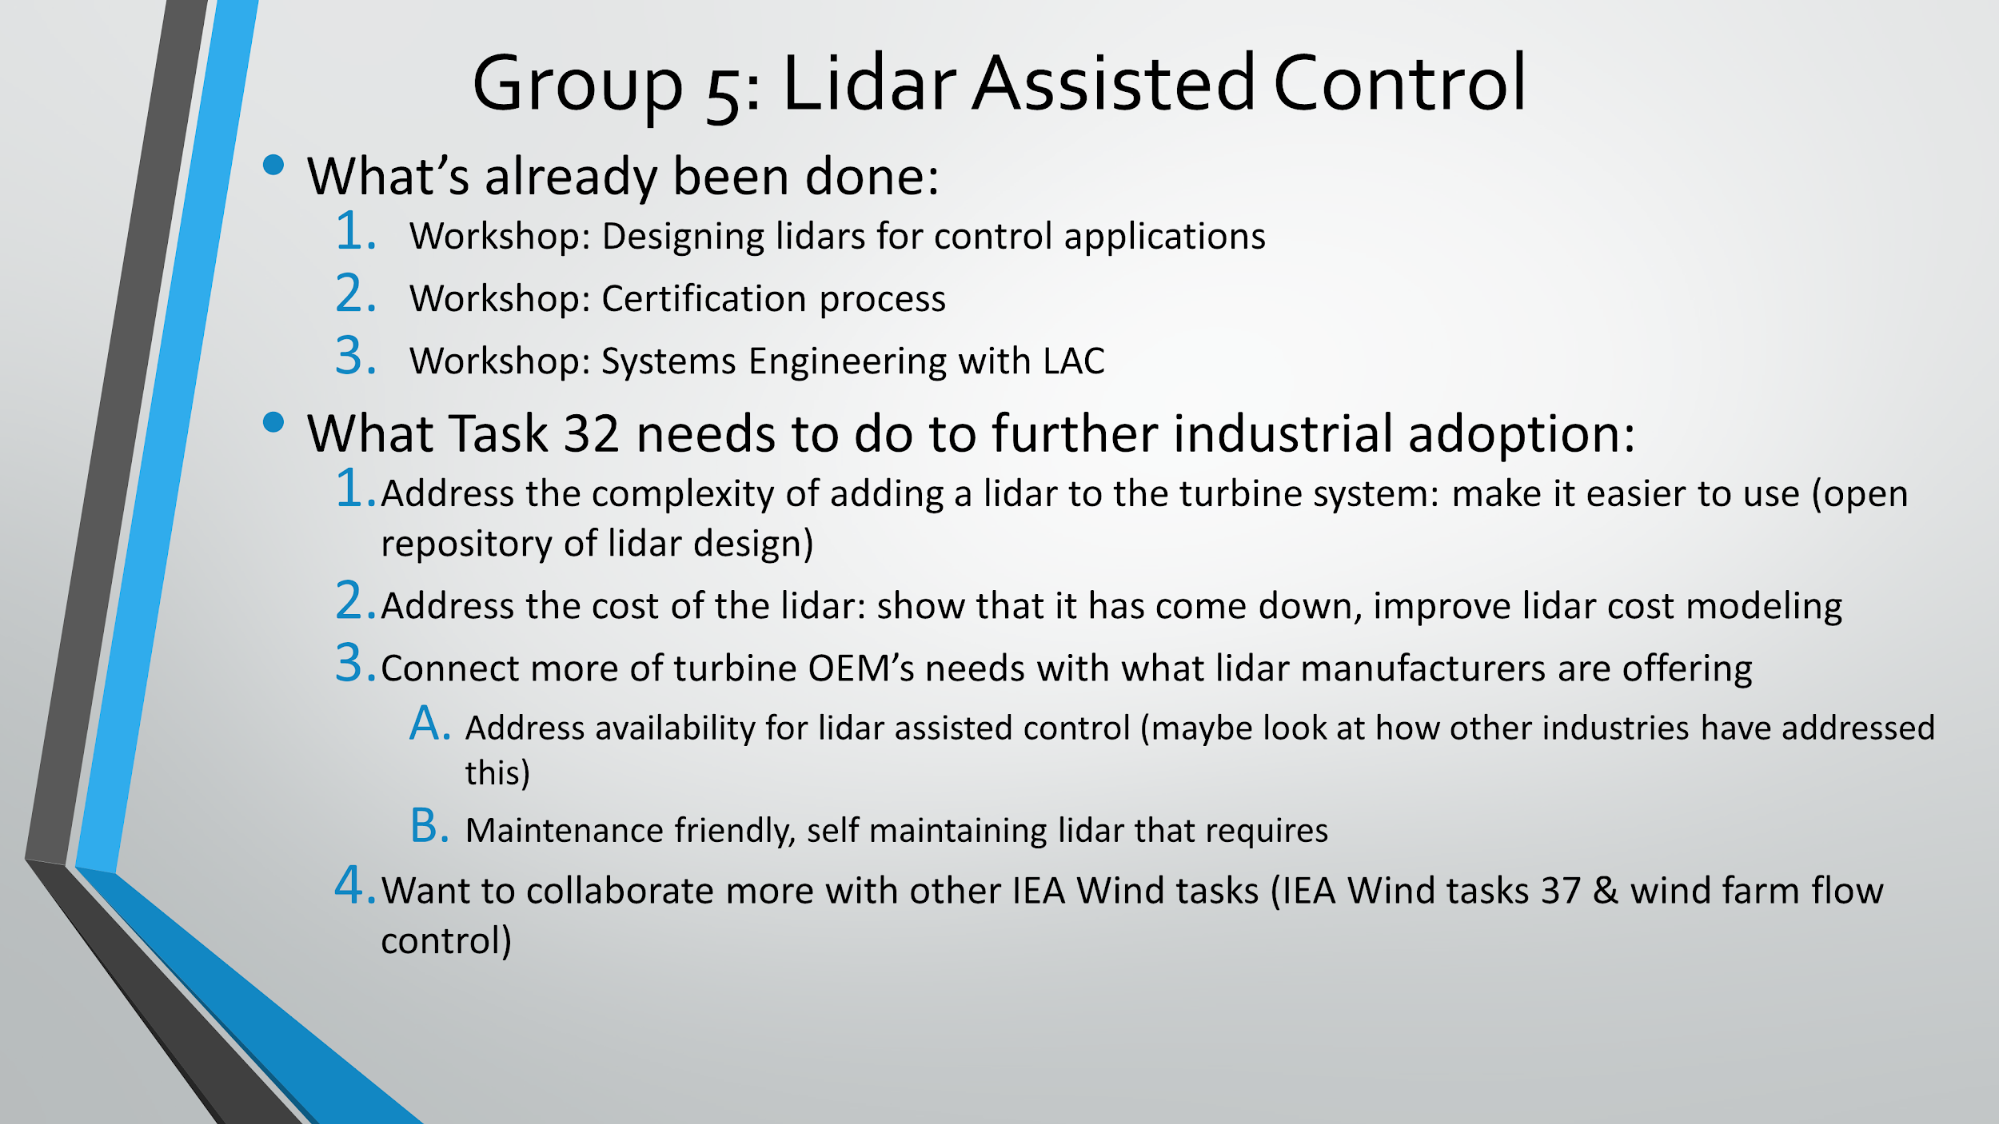
\includegraphics[width=0.85\textwidth]{figures/day3-LAC.png}
    }
    \caption{How Task 32 can enable adoption of lidar-assisted control of wind turbines and plants}
    \label{fig:day3-LAC}
\end{figure*}


\end{document}
